%%%%%%%%%%%%%%%%%%%%%%%%%%%%%%%%%%%%%%%%%%%%%%%%%%%%%%%%%%%%%%%%%%%%%%%%%%%%%%%
% This template is distributed with ABSOLUTELY NO WARRANTY.
% It serves as a guideline and constitutes a basic structure for a
% thesis/dissertation. The user assumes full responsibility for formatting
% and typesetting their document and for verifying that all the thesis
% requirements set by the University of Tennessee are met. Please refer to the most
% recent UT thesis guide (http://web.utk.edu/~thesis/thesisresources.shtml)
% or contact the thesis consultant (http://web.utk.edu/~thesis/).
% Please report any bugs to the thesis consultant.
%%%%%%%%%%%%%%%%%%%%%%%%%%%%%%%%%%%%%%%%%%%%%%%%%%%%%%%%%%%%%%%%%%%%%%%%%%%%%%%
% O P T I O N S:
% 1. thesis/dissertation
% 2. monochrome
% 3. all options provided by the report class
\documentclass[dissertation,letterpaper,12pt]{utthesis} % thesis, one side
\input{Preamble}
% some alternatives are:
%\documentclass[thesis,monochrome,letterpaper,12pt]{utthesis} %thesis, one side, monochrome text
%\documentclass[thesis,twoside,letterpaper,12pt]{utthesis} % thesis, two side
%\documentclass[thesis,monochrome,twoside,letterpaper,12pt]{utthesis} % thesis, two side, monochrome text
% for a dissertation, replace the thesis option by dissertation:
% \documentclass[dissertation,letterpaper,12pt]{utthesis} . . .
\renewcommand{\baselinestretch}{1.5} 	 % line Spacing
%%%%%%%%%%%%%%%%%%%%%%%%%%%%%%%%%%%%%%%%%%%%%%%%%%%%%%%%%%%%%%%%%%%%%%%%%%%%%%%
% TO DO: FILL IN YOUR INFORMATION BELOW - READ THIS SECTION CAREFULLY
%%%%%%%%%%%%%%%%%%%%%%%%%%%%%%%%%%%%%%%%%%%%%%%%%%%%%%%%%%%%%%%%%%%%%%%%%%%%%%%
\title{Optimization of Scintillator based Radiation Portal Monitors}
\author{Matthew J. Urffer}
\date{December, 2013}
\copyrightYear{2013} 
\graduationMonth{December}
\majorProfessor{Laurence F. Miller}
\keywords{Neutron Detectors, Radiation Portal Monitors, GEANT4, MCNPX, Simulation}
\college{Engineering}
\dept{Nuclear Engineering}
\university{The University  of Tennessee, Knoxville}
\viceProvost{Carolyn R. Hodges}
\major{Nuclear Engineering}
\degree{Doctor of Philosophy}
\college{Engineering}
\dept{Nuclear Engineering}
\university{The University  of Tennessee, Knoxville}
\numberOfCommitteeMembers{3}
\committeeMemberA {Lawrence H. Heilbronn}
\committeeMemberB {Dayaker Penumadu}
\committeeMemberC {Ronald E. Pevey}
%%%%%%%%%%%%%%%%%%%%%%%%%%%%%%%%%%%%%%%%%%%%%%%%%%%%%%%%%%%%%%%%%%%%%%%%%%%%%%%
% LOAD SOME USEFUL PACKAGES
%%%%%%%%%%%%%%%%%%%%%%%%%%%%%%%%%%%%%%%%%%%%%%%%%%%%%%%%%%%%%%%%%%%%%%%%%%%%%%%
\graphicspath{{tmp/}{figures/}{figures/eps/}{figures/pdf/} }% specify the path where figures are located
\usepackage{fancyhdr}                   % fancy headers and footers
\usepackage[inactive]{srcltx}		 	% necessary to use forward and inverse searching in DVI
\usepackage{relsize}                    % font sizing hierarchy
%%%%%%%%%%%%%%%%%%%%%%%%%%%%%%%%%%%%%%%%%%%%%%%%%%%%%%%%%%%%%%%%%%%%%%%%%%%%%%%
  \newcommand{\rangeSimGeo}{The simulation is a \SI{10}{\m} box of polystyrene completed with the GEANT4 toolkit.  More details of the simulation can be found in \autoref{sec:range-simulation}. } 
%%%%%%%%%%%%%%%%%%%%%%%%%%%%%%%%%%%%%%%%%%%%%%%%%%%%%%%%%%%%%%%%%%%%%%%%%%%%%%%
\begin{document}
    \pagenumbering{alph} % this is needed to clear certain issues with the hyperref package
    %
    %
    \addToPDFBookmarks{0}{Front Matter}{rootNode} % create a root node named "Front Matter" in the pdf bookmarks
    \addToPDFBookmarks{1}{Title}{a} % add a pdf bookmark to the title page
    \maketitle
    %
    \pagenumbering{roman}
    \setcounter{page}{2}
    %
    \addToPDFBookmarks{1}{Dedication}{b} % add a pdf bookmark to the dedication page
    \chapter*{}
\begin{center}
{\centering \textit{To my family and friends}}
\vspace{2 cm}
\begin{figure}[h]
\centering
\includegraphics[width=0.5\textwidth]{tryScience}
\end{figure}
\end{center} 

 % include the dedication
    %
    \addToPDFBookmarks{1}{Acknowledgements}{c} % add a pdf bookmark to the acknowledgements page
    \chapter*{Acknowledgments}

This works would not have been possible without the support of various resources.
Dr. Miller has been an essential resource for bouncing ideas around while providing valuable insights and encouragement for this work.
I would also like to thank my committee members, Dr. Heilbronn, Dr. Penumadu, and Dr. Pevey, for their support and technical expertise that they have provided. 
The testing of films would not have been possible without the kind folks fabricating the materials, I would like to acknowledge the work of Dr. Mabe, Dr. Auxier II, and Dr. Uppal for their help and numerous conversations.

The academic portion of this would have never succeeded without the support from my friends and family. 
My mother and father, Lisa and Micheal, deserve special recognition of their support, encouragement and frank advice. 
Katie, Samuel, David, Isaac, Esther and Eli also deserve recognition for being spectacularly supportive siblings. 
Finally, I would like to thank the members of Knoxville Ultimate for being supportive and offering many great games.

Financial support from the Domestic Nuclear Detection Office (DNDO) through Award No. 003387891 is gratefully acknowledged. 
 Any opinions, findings, and conclusions or recommendations expressed in this material are those of the presenter and do not necessarily reflect the views of DNDO.
 % include the acknowledgements
    \addToPDFBookmarks{1}{Abstract}{d} % add a pdf bookmark to the title page
    \begin{abstract}
    \chapter*{Abstract}
\label{chap:abstract}
Alternative neutron detection technologies are required to replace the current He-3 based Radiation Portal Monitors (RPMs).
RPMs are placed at border crossings into the United States in order to detect special nuclear material that may be entering the United States illicitly.
Replacement technologies must fulfill the following criteria established by the Department of Homeland Security: 1) a neutron detection efficiency, 2) a gamma insensitivity, and 3) the performance of the detector should not suffer in the the presence of a strong gamma field.
Several candidate detector designs have been proposed, including boron lined straw tubes, boron trifluoride gas detectors, scintillating Li-6 doped glass detectors, and other Li-6 based scintillators.
Polymeric films containing Li-6 ranging from 15 to 300 microns have the ability to fulfill these criteria if suitably utilized.
There exists a need to model and optimize these detector designs in order to ensure that the best performance is obtained. 
For a typical detector the design involves maximizing the neutron-gamma discrimination, maximizing the physical detector configuration in order to ensure optimal use of the incident neutron spectra, and ensuring that the scintillation light generated can be collected.

A technique for using a pulse height discriminator for rejecting gamma interactions has been determined for polymeric films  ranging from 15 microns to 300 microns in thickness.
The basis of this technique has been attributed to the relative ranges of the secondary electrons of the Compton scattered electrons from the gamma interactions, compared to the ranges of the electrons from the reaction products of a neutron absorption.
The Compton scattered electrons from a photon interaction generally have energies in the hundreds of keV while the Li-6 reaction products have energies in the 10 keV range, which results in the most of the energy from Compton scattered electrons escaping a thin (250 microns or less) film.
Detailed Monte Carlo (GEANT4) simulations indicate that a desired film thickness is around 100 microns.

A replacement portal monitor has then been designed for layered polymeric films that effectively utilize the Li-6 in the detector material.
These layered detector designs consist of 100 micron, Li-6 fluoride loaded polymers that are encased in four millimeters of a wavelength shifter.
A genetic algorithm was used to optimize a layered detector design that is capable of meeting the replacement RPM criteria.
A design in which four cylindrical tubes was also simulated, which is also capable of meeting the replacement RPM criteria while using more Li-6 for the same interaction rate as a layered detector design.
The light collection of the layered detector assemblies was also determined by Monte Carlo simulation.
If two photomultiplier tubes are placed at the top and bottom of a fishtail light guide mounted on the top and bottom of the detector cabinet, eight precent of the optical photons generated in a 10 precent loaded polystyrene film can be collected, leaving an acceptable number of photons to create a signal.

    \end{abstract}
    %
    \pagenumbering{roman}
    \setcounter{page}{2}
    %
    \addToPDFBookmarks{1}{Table of Contents}{e}
    \tableofcontents % generate a table of contents
    %
    \addToPDFBookmarks{1}{List of Tables}{f}
    \listoftables % generate a list of tables
    %
    \addToPDFBookmarks{1}{List of Figures}{g}
    \listoffigures % generate a list of figures
    %
    \makenomenclature % OPTIONAL
    \addToPDFBookmarks{1}{Nomenclature}{h} % OPTIONAL
    \printnomenclature[1.25in] % OPTIONAL
    %
    \newpage
    \pagenumbering{arabic}
    \setcounter{page}{1}
    %%%%%%%%%%%%%%%%%%%%%%%%%%%%%%%%%%%%%%%%%%%%%%%%%%%%%%%%%%%%%%%%%%%%%%%%%%%
    % INCLUDE THE CHAPTERS STARTING WITH THE NOMENCLATURE IF PRESENT
    %%%%%%%%%%%%%%%%%%%%%%%%%%%%%%%%%%%%%%%%%%%%%%%%%%%%%%%%%%%%%%%%%%%%%%%%%%%
    %%%%%%%%%%%%%%%%%%%%%%%%%%%%%%%%%%%%%%%%%%%%%%%%%%%%%%%%%%%%%%%%%%%%%%%%%%%
%                                                                         %
%                         PROJECT INTRODUCTION                            %
%                                                                         %
%%%%%%%%%%%%%%%%%%%%%%%%%%%%%%%%%%%%%%%%%%%%%%%%%%%%%%%%%%%%%%%%%%%%%%%%%%%
\chapter{Introduction} 
\label{chap:Intro}
Radiation Portal Monitors (RPMs) are passive radiation detection systems implemented at over a thousand of border crossings, and are designed to determine if cargo contains any special nuclear material in a safe, nondestructive, and effective manner\cite{kouzes_neutron_2010}. 
However, the current technology used in RPMs for detecting neutrons emitted from special nuclear material use a rapidly diminishing resource, \iso[3]{He}, that cannot be economically replaced. 
The Department of Homeland Security (DHS) continues to fund research (through the Domestic Nuclear Detection Office (DNDO)) for the development of detector systems to detect radioactive material that could potentially be used to cause significant economic loss and loss of life.  
As a result of this research a number of alternative detection systems continue to be investigated with the most viable including: boron trifluoride filled proportional detectors, boron-lined proportional detectors, \iso[6]{Li} loaded scintillation glass fiber detectors, and \iso[6]{Li} plus scintillator-coated wavelength-shifting fiber detectors\cite{pnnl_18471,kouzes_neutron_2010}.  

Neutron detectors often utilize a material with a large thermal cross section for absorption, such as \iso[6]{Li} (\SI{940}{\barn}) or \iso[10]{B} (\SI{3,800}{\barn}).
When these materials absorb a neutron they usually disintegrate to produce ionized reaction products that in turn transfer their kinetic energy to electrons.
In the case of the $\iso[6]{Li}\left(n,\iso[3]{H}\right)\alpha$ reaction, the fission energy is distributed between a triton of energy \SI{2.73}{\mega\eV} and an alpha of energy \SI{2.05}{\mega\eV}.
In a proportional counter such as the \iso[3]{He} based detectors,the energy from the charged particles would ionize a gas, creating a voltage signal.
Scintillator detectors, on which this work is based, utilize the charged particle energy depositions to create electron excitations in the scintillating material which are then transferred by fluors and produce visible light, which is detected with a photomultiplier tube.

\section{Replacement Detector Criteria}
\label{sec:ReplacmentCriteria}
Pacific Northwest National Lab (PNNL) along with the DNDO have developed a set of specifications that that replacement RPMs must meet \cite{kouzes_neutron_2010, kouzes_neutron_1999}. 
In particular 1) an absolute neutron detection efficiency greater than \SI{2.5}{\cps\per\ng \iso[252]{Cf}} at \SI{2}{\meter} for a defined moderated  source, 2) an intrinsic gamma-neutron detection efficiency of one in a million, and 3) a gamma absolute rejection ratio for neutrons stating that the performance of the detector should not change by more than 10\% in a \SI{10}{\milli\roetgen\per\hour} gamma field.
These parameters are summarized in \autoref{tab:DHSCritera}.
\begin{table}
  \centering
	\caption{Replacement Portal Monitor Criteria}
	\begin{tabular}{m{8cm} m{6cm} }
  \toprule
	Parameter & Specification \\
	\midrule
  Absolute neutron detection efficiency & 2.5 cps/ng of \iso[252]{Cf} (in specified test configuration) \\
	Intrinsic gamma-neutron detection efficiency & $ \epsilon_{int,\gamma n}\leq 10^{-6}$ \\
	Gamma absolute rejection ratio for neutrons (GARRn) & $ 0.9 \leq \text{ GARRn }\leq$ 1.1 at 10 mR/h exposure \\
	Cost &  \$ 30,000 per system \\
  \bottomrule
	\end{tabular}
	\label{tab:DHSCritera}
\end{table}

The absolute neutron detection efficiency $\left (\epsilon_{abs,n} \right )$ is defined as the number of neutron pulses recorded by the detector normalized by the number of neutrons emitted by the source as shown in \autoref{eqn:absn}
\begin{align}
	\label{eqn:absn}
  \epsilon_{abs,n} = \frac{N_{nc}}{N_{ns}}
\end{align}
where \definevar{$N_{nc}$}{neutron count rate} and \definevar{$N_{ns}$}{neutron emission rate from the source}.
DNDO guidelines state that a \iso[252]{Cf} source placed \SI{2}{\meter} from the midpoint of the detector is to be used for the determination of the absolute neutron detection efficiency\cite{pnnl_18471}.
To reduce the gamma ray flux of \iso[252]{Cf} upon a candidate detector the source is shielded by at least \SI{0.5}{\cm} of lead, and the neutron spectrum is then moderated by \SI{2.5}{\cm} of polyethylene\cite{pnnl_18471}.
The intrinsic efficiency, which provides a measure of how sensitive the detector is to incoming radiation, is defined in \eqref{eqn:inteff}.
\begin{align}
  \label{eqn:inteff}
  \epsilon_{int} = \frac{\text{Number Counts Observed}}{\text{Number Quanta for Radiation Crossing Detector}}
\end{align}
The formulation presented in \eqref{eqn:inteff} is then adapted to photons, with the requirement that only one count per a million photons passing through the detector may be registered.
To account for this the subscript $\gamma n$ is added to the intrinsic efficiency \eqref{eqn:inteffNG}
\begin{align}
  \label{eqn:inteffNG}
  \epsilon_{int,\gamma n} &= \frac{P_{pc}}{P_{p\Phi}}
\end{align}
where \definevar{$P_{pc}$}{photon count rate} and \definevar{$P_{p\Phi}$}{photons crossing the detector}.
The intrinsic gamma-neutron detection efficiency is to be measured using either a \iso[192]{Ir}, \iso[137]{Cs}, or \iso[60]{Co} source placed at an appropriate distance so as to produce an exposure rate of \SI{10}{\milli\roetgen\per\hour} at the detector\cite{kouzes_neutron_1999}.
The final detector parameter, the gamma absolute rejection ratio (GARRn), characterizes the detector response in the presence of both a large gamma ray source (\SI{10}{\milli\roetgen\per\hour}) and a \iso[252]{Cf} neutron source (configured as it would be for an absolute neutron detection efficiency measurement).
This criteria, shown in \eqref{eqn:garrn}, implies that the performance of the detector should not change by more than 10\% in a strong gamma field\cite{kouzes_neutron_1999}.
\begin{align}
  \label{eqn:garrn}
  GARRn = \frac{ \epsilon_{abs,\gamma n}}{\epsilon_{abs,n}}
\end{align}

%%%%%%%%%%%%%%%%%%%%%%%%%%%%%%%%%%%%%%%%%%%%%%%%%%%%%%%%%%%%%%%%%%%%%%%%%%%
%                                                                         %
%                       CURRENT TECHNOLOGIES                              %
%                                                                         %
%%%%%%%%%%%%%%%%%%%%%%%%%%%%%%%%%%%%%%%%%%%%%%%%%%%%%%%%%%%%%%%%%%%%%%%%%%%
\section{Current Technologies}
\label{sec:CurrentTechnologies}
Currently a number of alternative technologies is being developed, but two of the most promising detector technologies are boron loaded straw fibers being developed by Proportional Technologies Inc. (Houston, TX) and LiF loaded ZnS(Ag) scintillator paddles being developed by Innovative American Technology (Coconut Creek, FL).
The boron straw tubes meet the count rate criteria with a gamma rejection rate estimated at \num{4e-9} while passing the GARRn \cite{kouzes_boron-lined_2012}.
LiF/ZnS(Ag) is a commercial inorganic scintillator that utilizes the alpha from the \iso[6]{Li} neutron capture to active the ZnS doped with silver (ZnS(Ag)). 
LiF/ZnS(Ag) has a high light output per neutron (\num{1.6E5} photons per neutron) with a decay time of approximately \SI{100}{\micro\second} and the maximum emission at \SI{450}{\nm} \cite{carel_w.e_inorganic-scintillator_2001}.
However, this material is opaque and therefore care needs to be taken with the light collection of a large area detector.
Innovative American Technology (IAT) has developed a design of a replacement RPM that utilizes LiF/ZnS(Ag), as shown schematically in \autoref{fig:IATRender} and in \autoref{fig:IATImage}.
Current testing indicates that this detector design will meet the DHS criteria\cite{kouzes_lithium_2010}.
\begin{figure}
  \centering
  \includegraphics[width=0.5\textwidth]{IATRender}
	\caption[Rendering of IAT Neutron Detector]{Modeled IAT detector that consist of four paddles.  The paddles are angled to expose a larger surface to the neutron flux\cite{pnnl_22228}.}
	\label{fig:IATRender}
\end{figure}
\begin{figure}
  \centering
  \includegraphics[width=0.75\textwidth]{IATImage}
	\caption[Photograph of IAT Neutron Detector]{Photograph of the developed IAT detector\cite{pnnl_22228}.}
	\label{fig:IATImage}
\end{figure}

%%%%%%%%%%%%%%%%%%%%%%%%%%%%%%%%%%%%%%%%%%%%%%%%%%%%%%%%%%%%%%%%%%%%%%%%%%%
%                                                                         %
%                       DEVELOPED SCINTILLATORS                           %
%                                                                         %
%%%%%%%%%%%%%%%%%%%%%%%%%%%%%%%%%%%%%%%%%%%%%%%%%%%%%%%%%%%%%%%%%%%%%%%%%%%
\section{Thin Film Scintillators}
\label{sec:DevelopedScintillators}
In addition to the inorganic scintillator LiF/ZnS(Ag), work is being completed at the University of Tennessee to construct thin film polymeric scintillators to be utilized in a layered detector design for replacement RPMs.
These films, either based on polystyrene (PS) or polyethylene naphthalate (PEN), are \iso[6]{LiF} containing polymers projected to be low cost, have high mechanical durability, and meet the detector criteria \cite{Sen_Composites,Mabe201329}.
These new materials have been characterized for their neutron performance and gamma discrimination abilities, a summary of which (as of May 2013) may be found in \autoref{chap:MeasuredFilmPerfomance}.
%%%%%%%%%%%%%%%%%%%%%%%%%%%%%%%%%%%%%%%%%%%%%%%%%%%%%%%%%%%%%%%%%%%%%%%%%%%
%                                                                         %
%                       OPTIMIZATION INTRODUCTION                         %
%                                                                         %
%%%%%%%%%%%%%%%%%%%%%%%%%%%%%%%%%%%%%%%%%%%%%%%%%%%%%%%%%%%%%%%%%%%%%%%%%%%
\section{Optimization Opportunities}
There exists a need to build predictive modeling capabilities of these detectors in order to optimize the detector performance.
For a particular material and neutron absorber the detector geometry can be optimized to maximize the energy deposited in scintillation material by charged particles relative to the energy deposited by photon interactions. 
This in turn permits one to maximize the recorded neutron interaction rate relative to recorded photon interaction rates by setting a lower level discriminator (LLD) above a threshold associated with energy deposited in the detector by photons.  
As the LLD is increased, the efficiency for detecting neutrons is diminished; however, the intrinsic efficiency for detecting neutrons relative to photons is dramatically increased. 
In addition, as the neutron flux is being moderated and absorbed by the RPM material there exist the opportunity to position the neutron absorber films to maximize the neutron count rate while minimizing the amount of material being used.
Finally, it is essential to ensure that the scintillation light can be collected efficiency.

%%%%%%%%%%%%%%%%%%%%%%%%%%%%%%%%%%%%%%%%%%%%%%%%%%%%%%%%%%%%%%%%%%%%%%%%%%%
%                                                                         %
%                       ORGINAL CONTRIBUTION                              %
%                                                                         %
%%%%%%%%%%%%%%%%%%%%%%%%%%%%%%%%%%%%%%%%%%%%%%%%%%%%%%%%%%%%%%%%%%%%%%%%%%%
\section{Original Contribution}
\label{sec:OrginalContribution}
The design of effective radiation portal monitors is a critical component in detecting and subsequent interdiction of special nuclear material.
Most researchers assume that adequate neutron-gamma discrimination can be achieved by the relatively low mass attenuation coefficient for polymers and taking advantage of the thinness of a detector, but for a common plastic based scintillator the detector would have to be less than \SI{160}{\nm} in order to have an interaction rate less than one in a million.
This work is unique in that the fundamental physics basis of the neutron-gamma discrimination is not attributed to the mass attenuation coefficient but rather to the ranges of the secondary electrons from photon interactions in the material depositing less energy than their neutron counterparts.
Current modeling work in large area neutron detectors focuses either with monolithic plastic slab geometries or with neutronic calculations that do not account for light collection and transport.
A layered detector design, while not unique, has not been optimized using a genetic algorithm for which the formulation or the problem is quite natural.
In addition, little modeling work has been completed on the performance of a radiation portal monitor including light transport, which is a large majority of this work.
This work seeks to develop a strategy for the optimization of thin film layered detector designs utilizing a genetic algorithm and determining the expected number of scintillation photons that can be collected on a PMT through simulation.


%%%%%%%%%%%%%%%%%%%%%%%%%%%%%%%%%%%%%%%%%%%%%%%%%%%%%%%%%%%%%%%%%%%%%%%%%%%
%                                                                         %
%                               DOCUMENT LAYOUT                           %
%                                                                         %
%%%%%%%%%%%%%%%%%%%%%%%%%%%%%%%%%%%%%%%%%%%%%%%%%%%%%%%%%%%%%%%%%%%%%%%%%%%
\section{Organization of Dissertation}
The layout of this document follows the optimization of the design from the detector material to the optimal placement of the material.
The physical basis for the detector is described in \autoref{chap:theory} where a brief introduction of nuclear interactions is considered along with charged particle interactions, scintillations, and optics.
Specific methods used in this work are then discussed in \autoref{chap:methods}.
These methods include the GEANT4 modeling, MCNPX and XSDRN modeling, and the optimization technique employed.
The application of these methods are presented in \autoref{chap:results}.
Finally, \autoref{chap:Conclusions} serves to summarize the various lessons of the detector design.
  		% Problem introduction
    \chapter{Theory}
\label{chap:theory}
Effective design of a radiation portal monitor should be guided by the physics guiding the processes of interest.
These fields include the interactions of neutrons with matter and their subsequent absorption, the study of charged particle interactions with matter, scintillation, and optics.
 
%%%%%%%%%%%%%%%%%%%%%%%%%%%%%%%%%%%%%%%%%%%%%%%%%%%%%%%%%%%%%%%%%%%%%%%%%%%
%                                                                         %
%                      NUCLEAR INTERACTIONS                          %
%                                                                         %
%%%%%%%%%%%%%%%%%%%%%%%%%%%%%%%%%%%%%%%%%%%%%%%%%%%%%%%%%%%%%%%%%%%%%%%%%%%
\section{Nuclear Interaction Mechanisms}
\label{sec:NuclearInteractions}
They are several nuclear interactions that are of interest for radiation portal monitors. These reactions are


%%%%%%%%%%%%%%%%%%%%%%%%%%%%%%%%%%%%%%%%%%%%%%%%%%%%%%%%%%%%%%%%%%%%%%%%%%%
%                                                                         %
%                      ENERGY SCALE AND RANGES                            %
%                                                                         %
%%%%%%%%%%%%%%%%%%%%%%%%%%%%%%%%%%%%%%%%%%%%%%%%%%%%%%%%%%%%%%%%%%%%%%%%%%%
\section{Charged Particle Interactions and Ranges}
\label{sec:InteractionsAndRange}
\input{theory/RnageEnergyTheory}

%%%%%%%%%%%%%%%%%%%%%%%%%%%%%%%%%%%%%%%%%%%%%%%%%%%%%%%%%%%%%%%%%%%%%%%%%%%
%                                                                         %
%                      SCINTILLATION MECHANICS                            %
%                                                                         %
%%%%%%%%%%%%%%%%%%%%%%%%%%%%%%%%%%%%%%%%%%%%%%%%%%%%%%%%%%%%%%%%%%%%%%%%%%%
\section{Scintillation Mechanisms}
\label{sec:ScintMechanics}
%%%%%%%%%%%%%%%%%%%%%%%%%%%%%%%%%%%%%%%%%%%%%%%%%%%%%%%%%%%%%%%%%%%%%%%%%%%
%                                                                         %
%                         Introduction to Scintillation                   %
%                                                                         %
%%%%%%%%%%%%%%%%%%%%%%%%%%%%%%%%%%%%%%%%%%%%%%%%%%%%%%%%%%%%%%%%%%%%%%%%%%%

Scintillation detectors (the detectors on which this work is based) utilize a scintillator to convert ionizing radiation into photons.
In inorganic scintillators these photons arise from excitations of electrons in the band gap of the material or dopant, while for organic scintillators the photons generally come from relaxations of aromatic rings in the molecule.
Typically the light emitted from the primary phosphor is of a wavelength that is not suitable for detection with a photomultiplier tube, so a secondary fluor is added to absorb and reemit the light at a more favorable wavelength for detection.
The process of scintillation in organic scintillators is explained in more detail in \autoref{sec:OrganicScinillators}, while the number of photons emitted for different types of ionizing radiation is discussed in \autoref{sec:PulseHeightDeficit}.

\subsection{Organic Scintillators}
\label{sec:OrganicScinillators}
An organic scintillator generally has a $\pi$-electron structure similar to that of \autoref{fig:benzePiStructure} with typical energy levels as shown in \autoref{fig:pielectron}.
An incoming electron (liberated from the energy deposition of the ionizing radiation) then excites one of the modes of the $\pi$-electron structure.
Higher singlet states rapidly (on the order of picoseconds) relax to the first singlet state, and excessive vibrational energy (populations of the vibrational sates) is lost.
Thus, after a short period of time the entire excitation population is in the $S_{10}$ state, and the decay of this state creates the prompt fluorescence.
\begin{figure}
	\centering
	\includegraphics[width=0.5\textwidth]{benzeneStructure}
	\caption[Example orbitals for Benzene]{Example electron orbitals for Benzene.  The distributed, non-localized electron structure of the bottom image is typically of that of scintillators.}
	\label{fig:benzePiStructure}
\end{figure}
\begin{figure}
  \centering
  \includegraphics[width=0.6\textwidth]{PiElectronSates}
  \caption[$\pi$ Electron Structure]{Typical $\pi$-electron structure of an organic molecule. The ground state of the molecule is shown as $S_0$, and excited single states are $S_1$, $S_2$ etc The triplet states are $T_1$, $T_2$, with the vibrational states as $S_{OO}$, $S_{01}$, $S_{02}$ and so forth. Figure from Wikipedia.}
  \label{fig:pielectron}
\end{figure}
The excitations of triplet states typically yield delayed scintillation events or phosphorescence.
An excited triplet states immediately decays to the $T_0$ state by internal degradation without a photon emission.
The $T_0$ state typically decays by interacting with another $T_0$ state in a $T_0 + T_0 \to S^* + S_0 + h\nu$ transition.
The excited singlet state $S^*$ then also decays to the $S_0$ state.
The $T_0 + T_0$ transitions is slower than direct singlet state de-excitations, and results in a slow component of the pulse, which can be used for pulse shape discrimination.

The light output of an organic scintillator can be empirically related to the energy deposition in the scintillator through the Birks equation \cite{birks_scintillations_1951}.
In the absence of any quenching it is assumed that the light output per unit length is directly proportional to the energy deposition per unit length \eqref{eqn:LONoQuench}
\begin{align}
  \label{eqn:LONoQuench}
    \frac{dL}{dx} = S_B\frac{dE}{dx}
\end{align}
where \definevar{$S_B$}{absolute scintillation efficiency} and \definevar{$\frac{dE}{dx}$}{linear stopping power} .
If quenching of the light from molecules damaged by the radiation is also assumed to be proportional to the energy deposition per track length, than the Birks equation can be written as \eqref{eqn:BirksEquation}
\begin{align}
  \label{eqn:BirksEquation}
    \frac{dL}{dx} = \frac{S_B\frac{dE}{dx}}{1+kB\frac{dE}{dx}}
    \end{align}
    where \definevar{$kB$}{Birks parameter} which accounts for the quenching of the light.
For low stopping powers (or particles with a very high energy) the light output per unit track length is linear as the quenching term can be neglected.
However, for particles with a large stopping power the light output along the track length becomes saturated by quenching.
This difference in the pulse height accounts for that difference in light output from a \SI{1}{\MeV} electron compared to a \SI{1}{\MeV} alpha.
The \textit{alpha to beta} ratio provides a measure of this effect, and for the GS20 glass is it typically around 0.23.
This effect is critical in the developed detectors are the reaction products of of the \iso[6]{Li} neutron absorption are both heavily charged particles subject to this effect.
Thus, while there is \SI{4.78}{\MeV} of reaction product energy released in the neutron absorption, the low alpha to beta ratio of the material limits the actual number of scintillation events compared to those produced by a \SI{4.78}{\MeV} beta (electron).

\subsection{Pulse Height Deficit}
\label{sec:PulseHeightDeficit}
The concept of alpha to beta ratio is extended for other charged ions as the pulse height deficit.
The pulse height deficit is defined as the number of photons produced per energy of the primary particle (usually a heavy charged ion) relative to the number of photons produced per energy by an electron of a similar energy.
This is measured as the difference between the energy of the heavy ion and its apparent energy from the pulse height.  
Several researchers have investigated the light output of scintillators in response to different types of ionizing radiation\cite{Verbinski_1968}.
\autoref{fig:lightYieldVerbinski} summarizes example results in which the pulse height deficit is apparent for the as the charged ions become heavier.
\begin{figure}
  \centering
  \includegraphics[width=\textwidth]{Verbinski_LightYield_AlpahCarbonProton}
  \caption[Light yield non-proportionality of anthracene]{Light yield non-proportionality of anthracene. For the same kinetic energy the protons produce more photons alpha, which in turn produces more photons than the  carbon ions. This is an example of the pulse height deficit. Data from \cite{Verbinski_1968}.}
  \label{fig:lightYieldVerbinski}
\end{figure}

An illustration of the energy deposition between the different particles resulting in the pulse height deficit is presented in \autoref{fig:ParticleTracks}.
The electrons, with their low stopping power and broad track structure deposit their energy over a broader range than do the heavy charged ions (which tend to have rather collimated tracks).
Thus, the heavy charged ions deposit a large amount of their energy in a small volume, completely ionizing that volume and inhibiting scintillation.
\begin{figure}
  \begin{subfigure}[b]{0.45\textwidth}
    \includegraphics[width=\textwidth]{alphaTrack_0}
    \caption{\SI{2.05}{\MeV} Alpha}
  \end{subfigure}% 
  ~
  \begin{subfigure}[b]{0.45\textwidth}
    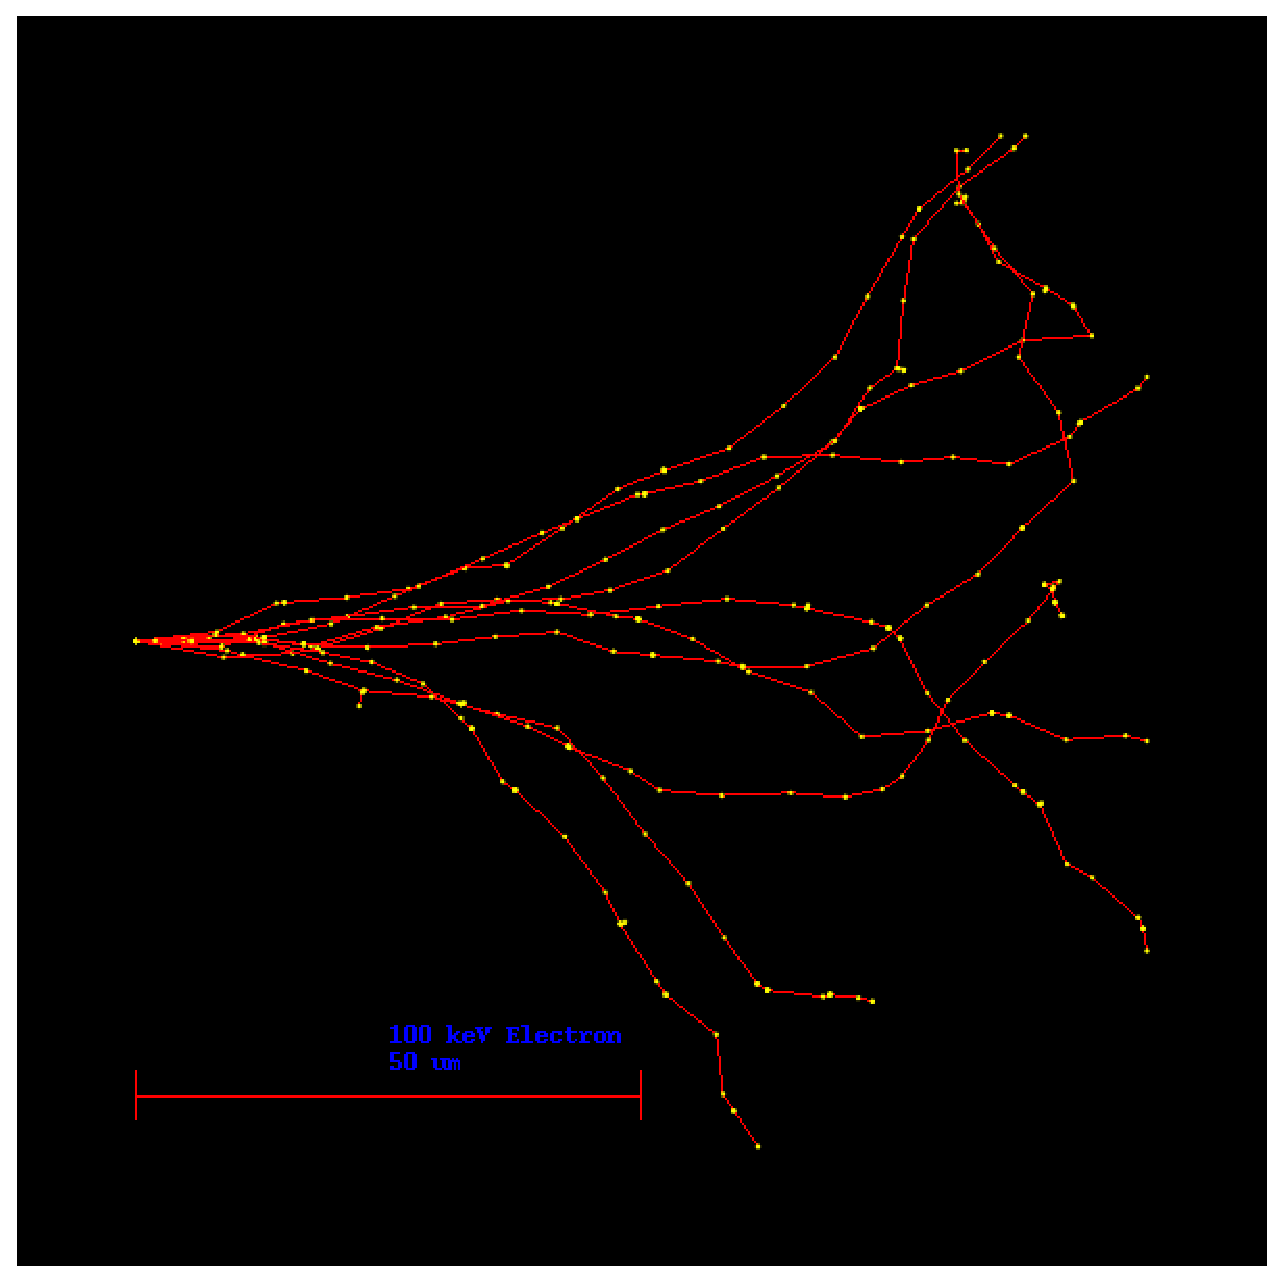
\includegraphics[width=\textwidth]{electronTrack_100keV_0}
    \caption{\SI{100}{\keV} Electron}
  \end{subfigure}
  
  \begin{subfigure}[b]{0.45\textwidth}
    \includegraphics[width=\textwidth]{electronTrack_50keV_0}
    \caption{\SI{50}{\keV} Electron}
  \end{subfigure}%
  ~
  \begin{subfigure}[b]{0.45\textwidth}
    \includegraphics[width=\textwidth]{tritonTrack_0}
    \caption{\SI{2.73}{\MeV} Triton}
  \end{subfigure}
  \caption[Particle Tracks of Alpha, Triton and Electrons]{GEANT4 simulated Particles tracks of a \SI{10}{\keV} electron, \SI{100}{\keV} electron, \SI{2.05}{\MeV} alpha, and \SI{2.73}{\MeV} triton.  The electron tracks are broader than the heavy ion tracks, resulting in a greater spread of the energy deposition and less quenching.}
  \label{fig:ParticleTracks}
\end{figure}

For a portal monitor scintillator the most likely charged particles would be alphas, tritons and electrons.
GEANT4 has the capability to simulate light quenching by setting an appropriate Birks parameter, and \autoref{fig:SimLightOutputQuench} presents GEANT4 simulated photon distributions in polystyrene with a PPO-POPOP fluor and an assumed light yield of 1,000 photons per MeV.
For highly energetic particles the electrons are almost an order of magnitude more efficient at creating light than the tritons, and about 90 times more efficient than the alphas, as shown in \autoref{fig:SimNumOP}.
However, it is unlikely that many electrons originating from \iso[60]{Co} interactions in the scintillator will have an energy in the \SI{1}{\MeV} range, more likely that they will be in the \SI{100}{\keV} range.
Thus, as shown in \autoref{fig:SimLightOutputQuench} the triton from the \iso[6]{Li} reaction will produce about an factor of five more photons than at \SI{100}{\keV}, and dominates the number of photons produced by the alpha particle.
\begin{figure}
  \centering
    \includegraphics[width=\textwidth]{SimLightQuench}
    \caption[Simulated Number of Optical Photons for Various Ions and Energies]{Simulated number of optical photons generated for electrons, alphas, tritons and \iso[7]{Li}.\LightQuenchSimGeo}
	\label{fig:SimNumOP}
  \end{figure}
  \begin{figure}
	\centering
    \includegraphics[width=\textwidth]{LightSim_AlphaTritonElectron}
  \caption[GEANT4 simulated light output of alpha, tritons and electrons in polystyrene]{Simulated optical photons distributions for the particles of interest in a portal monitor.  The energy of the electron was chosen to be the average energy deposited by \iso[60]{Co} in \SI{1}{\mm} of polystyrene. \LightQuenchSimGeo}
  \label{fig:SimLightOutputQuench}
\end{figure}

The pulse height deficit is computed by simulation of the charged particles and the corresponding electron.
This analysis yields a  pulse height deficit for the \iso[6]{Li} reaction as 8.5, and 27 for the \iso[10]{B}.
These results are summarized in \autoref{tab:PulseHeightDeficitSim}.
\begin{table}
  \caption[Simulated Number of Optical Photons for Selected Neutron Absorptions]{GEANT4 simulated number of optical photons produced for the \iso[10]{B} and \iso[6]{Li} neutron absorptions.  The scintillator is assumed to have a light yield of 1,000 photons per MeV}
  \label{tab:PulseHeightDeficitSim}
  \centering
  \begin{tabular}{c c c | c}
    \toprule
    & Particle & Photons Produced & Pulse Height Deficit \\
    \midrule
    \multirow{3}{*}{\iso[10]{B}} & $\alpha$ (\SI{1.78}{\MeV}) & 72 $\pm$ 8 &  \\
    & \iso[7]{Li} (\SI{1.02}{\MeV}) & 42 $\pm$ 8 & 27 \\
    & electron (\SI{2.78}{\MeV}) & 3,030 $\pm$ 160 & \\
    \hline
    \multirow{3}{*}{\iso[6]{Li}} & $\alpha$ (\SI{2.05}{\MeV}) & 87 $\pm$ 9 & \\
    & triton (\SI{2.75}{\MeV}) & 528 $\pm$ 23 & 8.5\\
    & electron (\SI{4.78}{\MeV}) & 5,250 $\pm$ 300 & \\
    \bottomrule
  \end{tabular}
\end{table}


%%%%%%%%%%%%%%%%%%%%%%%%%%%%%%%%%%%%%%%%%%%%%%%%%%%%%%%%%%%%%%%%%%%%%%%%%%%
%                                                                         %
%                      OPTICS and LIGHT TRANSPORT                            %
%                                                                         %
%%%%%%%%%%%%%%%%%%%%%%%%%%%%%%%%%%%%%%%%%%%%%%%%%%%%%%%%%%%%%%%%%%%%%%%%%%%
\section{Optics and Light Transport}
\label{sec:OpticsTheory}
Effective scintillator detectors collect as much light as emitted from the scintillator as possible.
In practice two effects limit the fraction of the emitted light collected; the optical self-absorption in the material and losses at the edges of the optical surfaces \cite{knoll_radiation_2009}.
The optical self-absorption of a scintillator is a material property in which photons are reabsorbed by the material.
This effect is important for large area scintillators and for scintillators which are not optically  clear, both of which apply to the developed polymeric scintillators.
Typically this effect is mitigated by the use of a wavelength shifting fiber in which the light is transferred to a material which has a much lower optical self-absorption.

Light collection of a scintillation event is emitted isotropically, and therefore only a very small fraction of the photons can travel directly to a photon detector surface.
The majority of the light must then be collected by reflecting back into the medium.
Snell's law governs the reflection of light at an optical boundary, and there are two cases to consider as shown in \autoref{fig:SnellsLaw} and described by Snell's Law, \eqref{eqn:SnellsLaw}
\begin{align}
	\theta_c = \sin^-1 \frac{n_1}{n_0}
	\label{eqn:SnellsLaw}
\end{align}
where \definevar{$\theta_c$}{critical angle}, \definevar{$n_1$}{index of refraction of the surrounding medium} and \definevar{$n_0$}{index of refraction of the scintillator}.
If the angle of incidence, $\theta$, is greater than the critical angle total internal reflection will occur.
When the angle of incidence is less than the critical angle particle reflection (or \textit{Fresnel} reflection) will occur and there will be partial transmission of the photons to the surrounding medium.
\begin{figure}
	\centering
	\includegraphics[width=\textwidth]{LightBoundary_SnellsLaw}
	\caption[Light Reflection at a Boundary]{Reflection of light at an optical surface is governed by Snell's law.  The fraction of light reflected back into the material is greatest at an angle of incident equal to $\theta_c$}
	\label{fig:SnellsLaw}
\end{figure}
To ensure that the light stays within the desired medium it is usually encased in a reflector, of which there are two types (\autoref{fig:SpecularDiffusive}).
A polished metallic surface (such as aluminized mylar) may be applied as a specular reflector which are generally better when the length is much longer than the thickness\cite{SaintGobain_DAM_2012}.
A diffusive reflector, such as teflon tape, is better for conditions when the detector is thick compared to its length \cite{knoll_radiation_2009}.
\begin{figure}
	\centering
	\includegraphics[width=\textwidth]{Riggi_SpecularDiffusive}
	\caption[Specular and Diffusive Reflection]{Specular reflection (a) in which the light in a single incoming direction is emitted as a single outgoing direction. The rough surface of a diffusive reflector (b), causes the light to be reflected at many angles. Figure from \cite{riggi_introducing_2011}.}
	\label{fig:SpecularDiffusive} 
\end{figure}

Photons that are emitted exactly along the direction of the scintillator will only be effected by the  absorption length of the material (typically on the order of \SI{100}{\cm} to \SI{400}{\cm} for optically clear materials\cite{SG_PlasticScint_2008}) while photons emitted in directions nearly normal to the direction of the scintillator will need to undergo thousands of reflections in order reach the PMT, which can double the length the photons must travel.
For perfect specular reflection it has been shown through simulation the the number of photons throughout a scintillating strip is only reduced by the optical absorption in that strip \cite{riggi_introducing_2011}.
In a realistic scintillator with a diffusive reflector the number of photons decreases by a factor of more than ten \SI{50}{\cm} from the origination of the photon\cite{riggi_introducing_2011}.

In the cases of a large scintillating detector, such as the one presented in this work, it  may be necessary to employ more than one PMT to collect the light.
In such cases the use of light pipes may enhance the collection efficiency. 
Light pipes are not without costs, however, as they are generally of a high index of refraction to maintain a high internal reflection, and it is desirable to optically match the surface at which the scintillator is to be viewed to prevent reflection.

The magnitude of the difficulty of collecting the optical photons is illustrated in \autoref{tab:PointSrcScintSlabResults}.
The simulation is a slab of PVT based scintillator (EJ-200) that is  \SI{200}{\cm} long, \SI{30}{\cm} wide, and of thickness between \SI{100}{\um} to \SI{1}{\cm} with perfectly polished sides so that the only interactions will be specular reflection due to Snell's law.
The geometry of this simulation is shown in \autoref{fig:WLSFiberSimGeo}.
While this simulation is not entirely representative of the light production (a uniform volumetric distribution would more accurately reflect the production in the scintillator) and the boundary conditions (perfectly smooth, polished surfaces are unrealistic), it demonstrates that there is a large reduction in the light collection due to having a thin detector.
It is also observed for the thin films that the distance from the PMT to the origination of the light has little effect as the rays need to start out nearly perpendicular to the PMT surface.
\begin{table}
	\caption[Fraction of Photons Detected from a Point Source on a single PMT]{Fraction of photons detected on a single PMT in a slab of various thickness from a point source located \SI{25}{\cm} and \SI{50}{\cm} from the detector.  The optical properties simulated are of that of a PVT based scintillator with an optical attenuation length set to \SI{200}{\cm}.}
	\label{tab:PointSrcScintSlabResults}
	% Data for this table may be found on pg. 30 of the third lab notebook
	\begin{tabular}{c | c  c}
	\toprule
	Slab Thickness & Fraction Collected (\SI{50}{\cm}) & Fraction Collected (\SI{25}{\cm}) \\
	\midrule
	\SI{100}{\um} & 1.1\% & 1.1\% \\
	\SI{220}{\um} & 1.3\% & 1.7\% \\
	\SI{460}{\um} & 1.5\% & 1.9\% \\
	\SI{1}{\mm} & 2.2\% & 2.8\% \\
	\SI{2.2}{\mm} & 3.5\% & 4.2\% \\
	\SI{4.6}{\mm} & 5.1\% & 6.2\% \\
	\SI{1}{\cm} & 6.3\% & 7.3 \% \\
	\bottomrule
	\end{tabular}
\end{table}
\begin{figure}
	\centering
	\includegraphics[width=\textwidth]{GEANT4AnnotatedGeo_WLSGeo}
	\caption[Thin Slab Light Collection Geometry]{Geometry of a the light collection in a thin scintillating slab. The material is a PVT based scintillator, with perfectly polished surfaces. Three optical photon events (represented by the green lines) are shown. The PMT's are considered to the the face of the material.}
	\label{fig:WLSFiberSimGeo}
\end{figure}
  		% Phyics Theory
    \chapter{Methods}
\label{chap:methods}
In the design of a detector the theory must be supplemented by accurate models of the complex interactions in the radiation portal monitor to determine the performance.
Once the performance of a design has been determined a method must be chosen for how to optimize the design to  ensure the best use of the materials while meeting the performance criteria.
Three models of the detector physics are employed; two Monte Carlo based methods and one deterministic method.
The deterministic model, XSDRN, solves a discretized one dimensional Boltzmann transport equation, and is described in \autoref{sec:XSDRNModel}.
Probabilistic models follow the path of individual neutrons with interactions based on the probability of a given event occurring.
Such codes are also known as Monte Carlo models, for which MCNPX (described in \autoref{sec:MCNPXModel}) and GEANT4 (described in \autoref{sec:G4Intro}) are well known examples.
MCNPX is employed for detailed neutronic modeling, while GEANT4 is employed for optical photon simulations and detailed energy deposition calculations.

The optimization of the detector is completed by a genetic algorithm using the XSDRN model to quickly simulate a large number of geometries.
Small perturbations on these geometries are then completed with the MCNPX model to ensure that the results are accurate and that true convergence has been reached.
The genetic algorithm is introduced in \autoref{sec:GAIntro}.

\section{Pulse Height Dissemination}
\label{sec:PulseHeightDiscrm}
\input{methods/PulseHieghtDiscr.}

\section{MCNPX Modeling}
\label{sec:MCNPXModel}
% MCNPX Model of the interaction rate
The performance of films is simulated in MCNPX, a Monte Carlo transport code\cite{pelowitz_mcnpx_2006}.
The geometry is as in the PNNL reports, namely a nano-gram of \iso[252]{Cf}  encased in \SI{0.5}{\cm} of lead and \SI{2.5}{\cm} of HDPE. 
The size of the RPM8 is \SI{12.7}{\cm} deep, by \SI{30}{\cm} wide and \SI{2}{\m} tall.
The interaction rate, $I_{\text{sim}}$ provides the total number of simulated neutron interactions in the detector and is calculated using the a cell flux tally in MCNPX and a tally multiplier card.
The reaction rate $\iso[6]{Li}\left(\text{n},\text{t}\right)\alpha$ can be calculated by then applying the appropriate input for the FMn card and using an F4 card to calculate $\phi(E)$.
This is in accordance with the direct evaluation of the PNNL criteria, which require a absolute neutron count rate of \SI{2.5}{count\per\second\per\nano\gram\iso[252]{Cf}}.
Note that in this calculation the source strength is set to be \SI{1}{\nano\gram} \iso[252]{Cf}, which has a neutron emission rate of \SI{2.3E3}{neutron\per\second}.
\begin{align}
  \label{eqn:RPM8InteractionRate}
  I_{\text{sim}} &= S_0 I \\
  &= \SI{2.3E3}{neutron\per\second} I
\end{align}
However, not all of these interactions will lead to counts above the pulse height discriminator setting necessary for meeting the gamma intrinsic efficiency.
This is corrected for by scaling $I_{\text{sim}}$ by the fraction of counts, $\eta$, that occur above the gamma LLD \eqref{eqn:FractionOfCountsDefination}, \eqref{eqn:RPMCountRate}.
\begin{align}
  \label{eqn:FractionOfCountsDefination}
  \eta \equiv \frac{\int_{MLLD}^\infty p(x)dx}{\int_0^\infty p(x)dx}
\end{align}
\begin{align}
 \label{eqn:RPMCountRate}
 \text{Count Rate} &= I_{\text{sim}} \eta
\end{align}
 
The MCNPX model was benched marked for characterized samples in the in house \iso[252]{Cf} neutron irradiator by simulating the interaction rate and comparing it to the measured count rate.
These results are summarized in \autoref{tab:MCNPXVal}.
It should be noted that the interaction rate is not directly the count rate as an interaction needs to have its scintillation photons collected in order to be a count. 
One would then expect the simulated interaction rate to be a few percent higher than the measured count rate.
In addition the polymeric sample composition is determined before pressing or casting providing a means for the uncertainty of the composition.
The relative error is defined as $(sim-obs)/obs)$.
\begin{table}
	\centering
	\caption[MCNPX Neutron Validation Results]{Comparison between simulated neutron interaction rate and measured count rate. It is expected that some of the uncertainity in the fabricated samples comes from not knowing exactly the amount of \iso[6]{Li} in the film, as it is determined before casting or pressing.}
	\label{tab:MCNPXVal}
	\begin{tabular}{m{4cm} | p{3cm} p{3cm} p{2cm}}
		\toprule
			Sample & Simulated Interaction Rate & Measured Count Rate & Relative Error \\
		\midrule
			GS20 & 424  & 428 & 0.7\%  \\ 
			PS 30\% LiF \SI{50}{\um} &  56 & 51 & 9.5\% \\
			PS 30\% LiF \SI{25}{\um} & 108 & 96 &13\%  \\
			PEN, 10\% LiF, \SI{110}{\um} & 75.1 & 70 & 7\% \\
			EJ426 HD2 & 226 & 224 & 0.8\% \\
		\bottomrule
	\end{tabular}
\end{table}

The gamma irradiator fluence was calibrated by measuring the dose rate are various positions, and then simulating the dose rate in MCNPX.
The results of this study are shown in \autoref{tab:MCNPXPhotonFluxVal}, and in general good agreement is observed between the simulation and the measurement.
In some cases where the simulated dose rate is higher may be due to uncertainty in the exact location of the probe in the measurement.
\begin{table}
	\centering
	\caption[MCNPX Photon Dose Rate Validation Results]{Comparison between simulated dose rate and measured dose rate.}
	\label{tab:MCNPXPhotonFluxVal}
	\begin{tabular}{c  c |c  c}
		\toprule
		\multicolumn{2}{c}{Measured} & \multicolumn{2}{c}{Simulated} \\
		Distance  & Dose Rate & Distance & Dose Rate \\
		\midrule
		\SI{10.2}{\cm} & \SI{10}{mRem \per h} & \SI{10.2}{\cm} & \SI{10.3}{mRem \per h} \\
		\SI{13}{\cm} & \SI{5.5}{mRem \per h} & \SI{12.8}{\cm} & \SI{5.4}{mRem \per h} \\
		\SI{28}{\cm} & \SI{2}{mRem \per h} & \SI{28}{\cm} & \SI{1.8}{mRem \per h} \\
		\bottomrule
	\end{tabular}
\end{table}


\section{XSDRN Modeling}
\label{sec:XSDRNModel}
% XSDRN Model of the RPM
The XSDRN model was a simplified model of the RPM along an axis through the midpoint of the RPM.
A $S_n$ of 16 was used for the quadrature, and convergence for the flux was set at \SI{1E-7} for the inner iterations.
Only two types of materials were simulated in the XSDRN calculation; a detector material containing the \iso[6]{LiF} and a moderating material of polystyrene.
A 44 group neutron cross sections of each of these materials were processed using NITWAL \cite{NITAWL_2011} (without any resonance regions) assuming an infinite, homogeneous medium for simplicity.
The XSDRN model consisted of a multi-group isotropic boundary source on the left most boundary on the RPM, with the values for this flux calculated by an MCNPX simulation.
A MCNPX calculation was used to determine the neutron flux incident upon the left most side of the RPM, and then this flux was input as the surface boundary flux condition in XSDRN.
The number of neutron absorptions was calculated using an activity flag in the XSDRN model.
The fitness function for this model was implemented as the activity normalized the number of detector layers.
The number of layers was chosen as the normalization factor instead of the actual mass of absorber to allow for different film compositions to be simulated more readily.

The comparison between the MCNPX simulation and the XSDRN is shown for some of the samples in \autoref{tab:10GenomeXSDRNMCNPXCompare} and \autoref{tab:20GenomeXSDRNMCNPXCompare}, where the change in rank is computed by rank of the MCNPX model versus the rank of the XSDRN model.
It is observed that the XSDRN model preformed fairly closely to the MCNPX model, but tended to over predict and favor geometries that had repeated layers and clusters.
This was very noticeable when the geometries started with a neutron absorber layer this is attributed to the breakdown of the diffusion equation in a strongly absorbing medium near a source.
Some stratification of the results were also observed, leading to the conclusion that the XSDRN calculations should only be used as a general guide.
More details are available in the simulation code base, summarized in \autoref{sec:garpm8opt}.
\begin{table}
  \caption[10 Genome Length RPM Model]{10 Genome Length RPM Model Interactions rates}
  \label{tab:10GenomeXSDRNMCNPXCompare}
  \begin{tabular}{c c | c c | c}
    \toprule
    Genome & Activity & Interaction Rate & Rank Change \\
    \midrule
  0011010000& 9.30 &  3.82 & $\downarrow$ 13 \\
  0110100000 & 10.50  &  3.81 & 0 \\
  0101010000 & 10.12  & 3.79 & $\downarrow$ 7 \\
 0101100000 &  & 3.79 & $\downarrow$ 1\\
  0011100000 & 9.63 &  3.77 & $\downarrow$ 3 \\
    \bottomrule
  \end{tabular}
\end{table}
\begin{table}
  \caption[20 Genome Length RPM Model]{20 Genome Length RPM Model Interactions rates}
  \label{tab:20GenomeXSDRNMCNPXCompare}
  \begin{tabular}{c c | c c | c}
    \toprule
    Genome & Activity  & Interaction Rate & Rank Change \\
    \midrule
  00100101000000000000 & 7.77 & 3.79 & $\downarrow$ 19 \\
  00011000100000000000 &  & 3.78 &  \\
  00011000010000000000 &  &  3.76 &  \\
  00110001000000000000 &  &  3.69 & $\downarrow$ 15\\
  01011010010000000000 & 23.46 & 3.66 & $\uparrow$ 1\\
    \bottomrule
  \end{tabular}
\end{table}


\section{GEANT4 Modeling}
\label{sec:G4Intro}
GEANT4 is a free toolkit for the simulation of particles as they travel through matter\cite{agostinelli_geant4simulation_2003}.
In general two types of applications were authored with the GEANT4 toolkit; ranges along with energy deposition and light transport.
All of the applications shared a common electromagnetic physics list based on the Livermore data set, and a cross section driven hadron physics list was used for the neutron interactions.
Ions were transported with the general ion physics list which contains detailed alpha and triton models.
Optical photons were transported with the default Optical Photon physics list.
More details on the GEANT4 toolkit may be found in \autoref{chap:G4Intro}.

\subsection{Energy Deposition Simulations}
\label{sec:EnergyDeposition}
The GEANT4 toolkit has the ability to track the energy deposition in different materials as well as the tracking of electrons to a least \SI{1}{\keV}\cite{agostinelli_geant4simulation_2003}.
It is proposed to represent the detector geometry as a single layer of neutron absorbing thin polymeric film mounted on top of a non-scintillating material (PMMA).
For simplicity, the initial events for runs will be chosen by setting up a particle gun for thermal (\SI{0.025}{\eV}) neutrons upon the detector and for both gammas resulting from a \iso[60]{Co} decay.
\begin{figure}
  \includegraphics[width=\textwidth]{GEANT4AnnotatedGeo_EnergyDepEvent}
	\caption[GEANT4 Energy Deposition Geometry]{GEANT4 Geometry for the Simulation of Energy Deposition. What is shown are 10 photons from a \iso[60]{Co} source impingement upon a \SI{2}{\cm} thick detector.  The photon tracks are shown in yellow, while the electron tracks are shown in red.}
	\label{fig:EDepSimGeo}
\end{figure}
It is expected that the the Livermore data-driven parameterized electromagnetic physics will be necessary to calculate the ionizing energy deposition, extending the standard electro-magnetic physics down to \SI{1}{\kilo\eV}.
The neutron interactions will be simulated with a hadronic modules, using the \verb+HP+ flavored modules to use the ENDF cross sections to calculate the interaction rates.

\subsubsection{Energy Deposition Validation}
The validation of this GEANT4 simulation was completed by reproducing the single collision energy loss in water as well as comparing  the spectral shapes and averages of simulated and measured spectra.
The reproduction of the single collision energy loss will ensure that the electron physics are implemented correctly, while the simulation of the polymeric film energy deposition allows the user to gain confidence that the correct tracking and binning analysis has been implemented.

The simulation was validated by reproducing the single collision energy loss for water as well as comparing spectra shapes and averages of simulated spectra to the measured spectra.
The single collision energy loss spectra for water that was simulated is shown in \autoref{fig:SingleCollisionELossWater}.
In general there was excellent agreement between the simulated energy spectra and a previously published spectra\cite{turner_comparative_1982}, with the simulated spectra having much better resolution than the reference did not.
It is thought that this is due to the water model in GEANT4 having better cross sections than the previously published spectra.
\begin{figure}[ht]
  \centering
  \includegraphics[width=\textwidth]{SingleCollisionEnergyLoss_300bins}
  \caption{Single Collision Energy Loss of Water. The simulated energy spectra matches that of Turner\cite{turner_comparative_1982}.}
	\label{fig:SingleCollisionELossWater}
\end{figure}

The validity of the GEANT4 simulation is determined by comparing the spectra shapes of measured spectra to simulated energy deposition.
Figure \ref{fig:spectraComparisonGamma} shows the comparison between the simulated energy deposition per incident photon from a \iso[60]{Co} source and the measured pulse height spectra from the \iso[60]{Co} irradiator per incident photon.
The energy calibration on the upper axis of the measured spectra was completed by finding the channel number at a given intrinsic efficiency and the corresponding energy at that intrinsic efficiency.
The energy of this feature on the measured spectra was then compared to the energy on the simulated spectra, with all of the values being within 10\%.
\begin{figure*}[ht]
	\centering
	\begin{subfigure}[b]{0.45\textwidth}
    		\includegraphics[width=\textwidth]{PS_EDepSim_Co60}
		\caption{GEANT4 Simulated Energy Deposition}
	\end{subfigure}%
	~
	\begin{subfigure}[b]{0.45\textwidth}
    \includegraphics[width=\textwidth]{PS_GammaCR-Binned-FluxNorm_20LiF_5PPO}
		\caption{Measured Pulse Height Spectra}
	\end{subfigure}%
	\caption{Comparison of the energy deposition and binned pulse height spectra for validation. The spectra have the same shape, indicating agreement. The fabricated films greater than \SI{600}{\um} were of poor optical quality and therefore their results are not shown.}
	\label{fig:spectraComparisonGamma}
\end{figure*}
The average energy deposition and average pulse height are shown in Figure \ref{fig:EDepLightYield}. 
With the average energy deposition on the left axis and the average light yield (pulse height) on the right axis, it is possible to compare the measurement and the simulation and agreement is observed.
\begin{figure*}[ht]
	\centering
	\begin{subfigure}[b]{0.45\textwidth}
    		\includegraphics[width=\textwidth]{G4EDep_LightYield_Co60}
		\caption{Gamma (\iso[60]{Co})}
	\end{subfigure}%
	~
	\begin{subfigure}[b]{0.45\textwidth}
    		\includegraphics[width=\textwidth]{G4EDep_LightYield_Neutron}
		\caption{Neutrons}
	\end{subfigure}%
	\caption{Average Energy Deposition and Measured Light Yield. The solid lines are calculated values and the red dots are measurements.}
	\label{fig:EDepLightYield}
\end{figure*}

\subsection{Optical Photon Simulatioins}
\label{sec:OpticalPhotonSims}
Optical photons were simulated in GEANT4 by creating an optical material property for each of the optical materials.
In general this involves setting the scintillation yield of the material, the resolution of the material, the optical photon absorbance of the film and the decay time.
It is also possible to set the Birks parameter of the material to simulate the light quenching of the material.
\autoref{tab:G4LightSimParam} enumerates several of the parameters used in the simulations.
\begin{table}
	\caption[GEANT4 Material Scintillation Parameters]{Parameters used in the simulation of optical process in GEANT4}
	\label{tab:G4LightSimParm}
	\begin{tabular}{c | c}
	\toprule
	Parameter & Value \\
	\midrule
	Birks Parameter &  \cite{Tretyak_2010} \\
	\bottomrule
	\end{tabular}
\end{table}
 and 

\subsection{Optical Photon Validation}
\label{sec:OpticalPhotonValidation}
The GEANT4 optical photon model was verified by measuring a detector and then simulating a similar detector in the GEANT4 toolkit. 
The comparison of the simulated entire  detection mechanisms (including the energy deposition, scintillation, and optical photon collection) to the a measured value provides confidence in the entire model; however, it should be noted that a validation of this type could allow for individual errors to miraculously cancel each other out.
Two cases where considered for the validation: 1) a sample mounted onto a PMT and 2) fabricated layered detectors that where  \SI{10}{cm} by \SI{15}{cm} by \SI{6}{cm} .
The single sample mounted on the PMT was used to establish the Birks constant for the material, and the fabricated layered detectors measurements were used to provide confidence of the ability to simulate a large scale detector system.

A single sample mounted on a PMT provides a simple geometry to validate the parameters used in the light transport simulations. 
The geometry consist of a sample mounted with a thin layer of optical grease to the PMT, and the entire assembly is wrapped with teflon grease.
This mimics the measurement of a sample mounted on a PMT, expect for the efficiency of the photocathode is not considered.

It should be noted that the Birks constant greatly impacts the number of optical photons generated and subsequently detected.
For GS20 a Birks constant of \SI{0.1}{\mm\per\MeV} produced 1,300 photons per neutron, while a Birks constant of \Si{0.01}{\mm\per\MeV} produces 6,900 optical photons per neutron.
Birks constants greater than \SI{0.01}{\mm\per\MeV} produce marginal increases in the number of optical photons produced; for example 8,600 photons per neutron were produced for a Birks constant of \SI{0.0001}{\mm\per\MeV}.
If agreement between the simulated and measured c

\section{Genetic Algorithm Introduction}
\label{sec:GAIntro}
Genetic algorithms provide a search technique analogous to biological evolution in which instead of searching from general to specific solutions, or from more simple to complex, genetic algorithms generate solutions by mutating and combining parts of the best previously known solutions.
At each step in the search for the best solution a collection of solutions called the current \textit{population} is refined by replacing members with solutions representing the offspring of the best individuals.
The goals is then to find the best solution to the problem as determined by some criteria, called the \textit{fitness function}.
The genetic algorithm typically consist of four tasks: creating an initial population, evaluating that populations fitness, selecting members of the current population to breed, and then applying genetic operators to the selected members to breed the new population. 
This is completed until either a maximum generation is reached or the desired fitness is achieved, as shown in \autoref{alg:GAOutline}.
\begin{algorithm}
  \caption{Genetic Program Outline}
  \label{alg:GAOutline}
  \begin{algorithmic}
    \WHILE{$error>goal$}
      \FORALL{$t\in F$}
        \STATE{Compute fitness}
      \ENDFOR
      \FORALL{$t\in F$}
        \STATE{Choose individuals based on fitness}
      \ENDFOR
      \STATE{Select individuals for next population}
      \STATE{Crossover selected individuals}
      \STATE{Mutate selected individual}
    \ENDWHILE
  \end{algorithmic}
\end{algorithm}

\subsection{Problem Representation}
The thickness of the RPM  (\SI{12.7}{\cm}) was divided into slices, where each slice could be either a detector slice or a moderator slice.
These slices of detector material (represented as a \verb+1+) or moderator material (represented as a \verb+0+) were append into a sequence.
This sequence of one's and zero's (or bit string) then completely represented the geometry of the RPM and formed the basis for all possible solutions to the optimization problem.
For example the sequence \verb+0001110010+ would represent a detector that had three moderator slices, three detector slices, another two moderator slices, and a final detector slice before a single moderator slice as the reflector.
Examples of two different genomes are shown in \autoref{fig:ExGeoGenomes}
\begin{figure}

  \caption[Example Geometries Genomes]{Example of Geometry Genomes}
  \caption{fig:ExGeoGenomes}
\end{figure}
In terms of genetic algorithms the set of all possible solutions is referred to as the \textit{genome}.
The length of the genome is thus the number of slices in the geometry, where a higher length genome allows for a more complicated geometry.
The initial population for the genetic algorithm was initialized to be random bit strings with equal probability of a slice being a detector slice or moderator.

\subsection{Population Selection}
Several different selection techniques are available to select the individuals from one population to reproduce in the next.
Among the most common are fitness proportional selection (roulette selection) and tournament selection.
Roulette selection occurs when the individuals are ranked by their fitness, and individuals are chosen by their fitness rank.
This is analogous to a roulette wheel where the space a candidate occupies on the wheel is proportional to its fitness.
Higher fitness individuals will occupy more space, and will thus have a higher probability of being selected.
Tournament selection is another selection technique in which a pool of solutions are chosen at random from the current population.
Within this tournament pool a fitness proportional selection will be used to select individuals for the next generation.
The fitness function will be explained in detail in \autoref{sec:FitnessFunc}.

\subsection{Genetic Operators}
Individuals selected for reproduction are subjected to genetic operators to breed the next generation. 
Genetic programs generally contain two genetic operators, crossover and mutation. 
Crossover serves to create new members of the population by interchanging the genetic material of two parents in which significant changes in the solutions are achieved. 
Mutation serves to slightly modify an existing solution. 

Crossover is defined in genetic programming as the swapping of genetic material from one individual to another.  
For bit strings several crossover operations are commonly used; they are 1) single point crossover, 2) two point crossover, and 3) uniform crossover.
An example of the crossover operations are shown in \autoref{fig:GeneticCrossover}.
In single point crossover a single point is selected on both parents genes and the genetic material between the two parents is swapped.
In two point crossover two points are chosen on the parents bit strings and the genetic material is swapped between the intervals.
Uniform crossover uses a set mixing ratio for which according to that ratio an individual bit will be interchanged between the two parents to yield the daughters.
\begin{figure}
  \begin{subfigure}[b]{0.3\textwidth}
    \includegraphics[width=\textwidth]{SinglePointCrossover}
    \caption{Single Point Crossover}
  \end{subfigure}
  ~
  \begin{subfigure}[b]{0.3\textwidth}
    \includegraphics[width=\textwidth]{TwoPointCrossover}
    \caption{Two Point Crossover}
  \end{subfigure}
  ~
  \begin{subfigure}[b]{0.3\textwidth}
    \includegraphics[width=\textwidth]{UniformCrossover}
    \caption{Uniform Crossover}
  \end{subfigure}
  \caption[Genetic Crossover Operations]{Genetic Crossover Operations. Images from Wikipedia}
  \label{fig:GeneticCrossover}
\end{figure}

Mutation is used to produce small, random changes in the genomes to maintain genetic diversity.
The mutation operation was chosen to be a simple bit flip in which a randomly chosen \verb+1+ or \verb+0+ in the geometry was flipped; for example \verb+001001010+ could be mutated to \verb+001001000+.
Generally the mutation rate is set very low (less than 2\%) in order to prevent the search for the solution to becoming simply a random search.
In this representation of the problem a mutation produces a very large change in the solution and the mutation rate was set even lower.

\subsection{Fitness Function}
\label{sec:FitnessFunc}
The fitness function defines the criteria for ranking solutions and probabilistically including them in the next generation.
The fitness function was chosen to count rate per mass of \iso[6]{Li}, provided that the geometry meet the total count rate criteria.
If it failed to meet the count rate criteria a zero fitness was returned \eqref{eqn:FitnessFun}.
\begin{align}
    \label{eqn:FitnessFun}
    f(\vec{x})
    = \begin{cases}
    0 & \text{if} \text{countRate}(\vec{x}) \leq \SI{2.5}{cps\per\nano\gram\iso[252]{Cf}} \\
    \text{countRatePerMass}(\vec{x})
    \end{cases}
\end{align}
Films that have excessive detector layers will be penalized by the normalization by the mass of \iso[6]{Li} that they contain, while favoring films that have the minimum number of detector layers that meet the count rate criteria and have a more effective utilization of the neutron flux which increase their count rate.

At this point it is instructive to make a note about the size of the solution space.
\autoref{tab:BitStringGeo} some of the these geometries are simple enough that the search space can be computed exhaustively.
\begin{table}
    \caption[Genome Bit String Geometries]{Bit String Simplified Geometry Descriptions}
    \label{tab:BitStringGeo}
    \centering
    \begin{tabular}{ c | c c}
     \toprule
     Genome Length&Slice Thickness&Possible Geometries \\
     \midrule
        5&2.54&31\\
        10&1.2700&1,023\\
        15&0.8467&32,765\\
        20&0.6350&1,048,575\\
        25&0.5080&33,554,431\\
        30&0.4233&\num{1.07E9}\\
        35&0.3629&\num{3.44E10}\\
        40&0.3175&\num{1.10E12}\\
    \bottomrule
    \end{tabular}
\end{table}
There are several salient features highlighted in \autoref{tab:BitStringGeo}.
For small genome lengths (less than 10) it is possible to exhaustively search the hypothesis space of possible solutions.
This is not possible for the larger genome lengths.
Therefore, efficient evaluation of the fitness function is necessary in order to evolve a reasonable number of solutions.
In addition the refinement in the details of the geometries increases linearly with the genome length while the size of the search space increases as $2^n$.
This suggest that a hybrid method of finding a basic geometry in a low search space and then preforming perturbations on that geometry will have a better performance than attempting to search the higher geometry solution space.
		% Modeling and GA Intro
    \chapter{Results}
\label{chap:results}

The basis for setting a pulse height discriminator to differentiate between neutron and gammas can be attributed to the secondary electrons and the difference in energy mechanisms as presented later.
However, the application to physical detectors has yet to be concretely formulated.
This section will serve to remedy that and present a pulse height discrimination scheme capable of discrimination between neutrons and gammas.

It is currently understood that the light output per path length in the film (which is directly proportional to the pulses collected on the PMT) is related to the stopping power of the radiation in the film material.
For a given material the stopping power of the film will be constant, and therefore the light output of the film can be found by integrating the light output per path length over the total length of the film.
It is then possible to conclude that the light output of a film is proportional to the energy deposited in the film.

Preferential energy deposition by reaction products from neutron interactions relative to gammas will enhance the discrimination by creating larger neutron light pulses than the gamma pulses, allowing for fewer neutron pulses to be classified as gamma pulses because they are below the MLLD.
Thus, neutron-gamma discrimination can be enhanced by optimizing the energy deposition in the film. 

\section{Energy Deposition}
%%%%%%%%%%%%%%%%%%%%%%%%%%%%%%%%%%%%%%%%%%%%%%%%%%%%%%%%%%%%%%%%%%%%%%%%%%%
%                                                                         %
%                     ENERGY DEPOSITION SIMULATIONS                       %
%                                                                         %
%%%%%%%%%%%%%%%%%%%%%%%%%%%%%%%%%%%%%%%%%%%%%%%%%%%%%%%%%%%%%%%%%%%%%%%%%%%

The average energy deposited by a neutron and gamma reaction was investigated for different film thickness to determine if an optimal thickness exits in a geometry similar to \autoref{fig:EDepSimGeo}.
\autoref{fig:SimEDep} shows that the energy deposition of the gamma quickly falls off as the films get thinner, while it isn't until the neutron films become on the order of the range of the triton that the energy deposition is impacted.
\begin{figure}
  \centering
  \includegraphics[width=\textwidth]{SimulatedEnergyDeposition}
  \caption[Simulated Energy Deposition and Film Thickness]{Simulated energy deposition and film thickness. As the films get thinner it is very unlikely for gamma events (and their secondary electrons) to deposition all of their energy, while above \SI{50}{\um} there is very little impact on the energy deposited by neutrons.\EnergyDepSimGeo}
  \label{fig:SimEDep}
\end{figure}

Interactions that occur near the edge of the film may have a large impact in the energy absorbed in the film for very thin films where a large fraction of the volume is within a mean free path of the surface of the detector material.
For example, for a \SI{25}{\um} film the range of the triton exceeds the thickness of the film.
The energy loss of interactions occurring near the edge of the film was investigated by simulating the energy loss for a large planar detector where the beam spot is \SI{3}{\mm} and the area of the detector face is \SI{10}{\cm}. 
The geometry for this simulation shown in \autoref{fig:EDepSimGeo}, with the interaction position defined to be distance to the first interaction of the beam in the material along the direction of the beam.
\autoref{fig:EDepPosSim} examines the impact of where the interaction took place in the film on the energy deposition.
It is observed that for neutrons events that take place within the center of the films tend to deposit a large majority of their energy in the film, while events that occur on the edge of the film have partial energy depositions in accordance with the ranges of the charged particles.
The Compton edge is observed at \SI{1}{\MeV} in the simulated photon energy deposition for the \SI{1}{\cm} film, as expected.
A secondary effect in having a backing material is also observed for photons in which there is a heightened energy deposition for interactions that occur in the film but near the boundary and electrons are back scattered into the detector material.
\begin{figure*}[ht]
	\centering
	\begin{subfigure}[b]{0.45\textwidth}
    		\includegraphics[width=\textwidth]{{posEDepCo600.025}.png}
		\caption{ \SI{25}{\um} Gamma (\iso[60]{Co})}
	\end{subfigure}%
	~
	\begin{subfigure}[b]{0.45\textwidth}
    		\includegraphics[width=\textwidth]{{posEDepCo6010.0}.png}
		  \caption{ \SI{1}{\cm} Gamma (\iso[60]{Co})}
	\end{subfigure}%
	
  \begin{subfigure}[b]{0.45\textwidth}
    		\includegraphics[width=\textwidth]{{posEDepneutron0.025}.png}
		\caption{ \SI{25}{\um} Neutron}
	\end{subfigure}%
	~
	\begin{subfigure}[b]{0.45\textwidth}
    		\includegraphics[width=\textwidth]{{posEDepneutron10.0}.png}
		  \caption{ \SI{1}{\cm} Neutron}
	\end{subfigure}%
	\caption[Simulated Energy Deposition and Position]{Simulated average energy depositions and the position of the first interactions. The beam is considered to be incident on position 0, and thus interactions that occur on the front of the film have a much higher probability depositing all of their energy. Events that occur on the edge of the film much less likely to deposit all of their available energy.}
	\label{fig:EDepPosSim}
\end{figure*}

\autoref{fig:simKinE} illustrates the simulated kinetic energy of secondary electrons from Compton scattering and from alpha and triton interactions.
It is observed that kinetic energy of the secondary electrons from the neutron reaction products have predominately energies in the kilo-volt range, while the Compton scattering electrons have energies in hundreds of kilo-volts range. 
However, it should be noted that there is only one secondary electron from a Compton scattering and multiple secondary electrons from the reaction products.
The kinetic energy distribution is broken down by the two reaction products in \autoref{fig:SecElecKinEDist}, while the relative number of secondary electrons is shown in \autoref{fig:ReacProdDist}.
It is apparent that the triton contributes more secondary electrons than heavier alpha, while they have similar energies of the secondary electrons.
\begin{figure}[ht]
    \centering
    \includegraphics[width=\textwidth]{NGSecElecKinEDist}
    \caption[Kinetic Energy of Primary Secondary Electron from Compton Scattering and Neutron Reaction Products]{The kinetic energy of the first secondary electron from Compton scattering with \iso[60]{Co} and from \iso[6]{Li} reaction products. The energy distribution of all of the electrons produced in the interactions is shown in \autoref{fig:ERangeAndDist}.\EnergyDepSimGeo}
    \label{fig:simKinE}
\end{figure}
\begin{figure}
 	\centering
  	\includegraphics[width=\textwidth]{AlphaTritonSecElecKinEDist}
	\caption[Kinetic Energy Distribution of Primary Secondary Electrons from the Neutron Reaction Products]{Kinetic energy distribution of the first secondary of the neutron reaction products (alpha and triton) from a \iso[6]{Li} interaction.  Most of the electrons have kinetic energies in the \SI{1}{\keV} range. \EnergyDepSimGeo}
	\label{fig:SecElecKinEDist}
\end{figure}
\begin{figure}
 	\centering
  	\includegraphics[width=\textwidth]{NeutronNumSecElec}
	\caption[Distribution of the Number of Secondary Electrons Produced Per Neutron Interaction]{Distribution of the Number of Secondary Electrons Produced Per Neutron Interaction. The alpha particle produces almost a factor of 16 less photons than the triton. \EnergyDepSimGeo}
	\label{fig:ReacProdDist}
\end{figure}

The average energy deposited was computed for each thickness and normalized by the incident energy for gammas by the Q-value of the reaction for neutrons, and is presented in \autoref{tab:FractionEDep}.
For thickness greater than \SI{150}{\um} there is little benefit in increasing the thickness of the film in terms of energy deposition by neutrons, since over 90\% of the energy is being deposited in the film.
\begin{table}
    \caption[Fractional Energy Deposition per Interaction for Various Thickness]{Fraction of total energy deposited per interaction of a neutron and the photons from \iso[60]{Co} in films of various thickness. The total energy deposited in a neutron event is \SI{4.78}{\MeV}, while the maximum energy deposited from a \iso[60]{Co} is \SI{1.33}{\MeV}.\EnergyDepSimGeo}
      \label{tab:FractionEDep}
	\centering
	\begin{tabular}{c | c c}
\toprule
	Thickness & Gamma Fraction & Neutron Fraction \\
\midrule
	\SI{15}{\um} & 0.010 & 0.531 \\
	\SI{25}{\um} & 0.013 & 0.634 \\
	\SI{50}{\um} & 0.017 & 0.782 \\
	\SI{150}{\um} & 0.032 & 0.927 \\
	\SI{300}{\um} & 0.052 & 0.964 \\
	\SI{600}{\um} & 0.087 & 0.982 \\
	\SI{1}{\mm} & 0.130 & 0.989 \\
	\SI{1}{\cm} & 0.425 & 0.998 \\
\bottomrule
	\end{tabular}

\end{table}

%%%%%%%%%%%%%%%%%%%%%%%%%%%%%%%%%%%%%%%%%%%%%%%%%%%%%%%%%%%%%%%%%%%%%%%%%%%
%                                                                         %
%                  Light Yield and Energy Deposition                      %
%                                                                         %
%%%%%%%%%%%%%%%%%%%%%%%%%%%%%%%%%%%%%%%%%%%%%%%%%%%%%%%%%%%%%%%%%%%%%%%%%%%
\section{Light Yield and Energy Deposition}
The energy deposition and light yield were also investigated by simulations in the GEANT4 environment for polystyrene based films.
These simulations (summarized in \autoref{fig:EDepLightYield}) show that as expected the light output was linear with the energy deposition.
The importance of the particles causing the scintillation events is due to the quenching of the light from heavy charged particles.
Thus, while the gammas from \iso[60]{Co} deposit  less energy than neutrons in a the same thickness of films, the light output is much higher per unit energy deposited.
\begin{figure}
 	\centering
  	\includegraphics[width=\textwidth]{EDepLightYield_Gamma}
		\caption[Energy Deposition and Light Yield in Polystyrene from Co-60 Photons]{Simulated energy deposition from gamma (\iso[60]{Co}) and the corresponding simulated light yield. \SimEDeLYGeo}
\end{figure}
\begin{figure}
 	\centering
  	\includegraphics[width=\textwidth]{EDepLightYield_Neutron}
  	\caption[Energy Deposition and Light Yield in Polystyrene from Neutrons]{Simulated energy deposition and light yield from neutron interactions.  \SimEDeLYGeo}
  \label{fig:EDepLightYield}
\end{figure}
However, it is instructive to look at the distributions of how many photons were created per event.
As the films become thicker and more of the triton energy is captured the response of the triton starts to dominate the alpha (\autoref{fig:NeutronPhotonsGenSim}), resulting in the number of photons peaking around 650 photons for this simulated sample.
For photons, shown in \autoref{fig:GammaPhotonsGenSim}, it is observed that the distribution is flat for very thick films, but for thinner films the probability is greatly increased for an event to generate a low number of photons.
\begin{figure}
  \centering
  \includegraphics[width=\textwidth]{Neutron_PhotonsGenerated_Sim}
  \caption[Number of photons generated from neutron interactions]{Simulated number of photons generated from neutron interactions.  For the \SI{10}{\um} film it is observed that the majority of the photons are generated by a partial energy deposition corresponding to the alpha particle, and this effect tappers off as the films get thicker. \SimEDeLYGeo}
  \label{fig:NeutronPhotonsGenSim}
\end{figure}
\begin{figure}
  \centering
  \includegraphics[width=\textwidth]{Gamma_PhotonsGenerated_Sim}
  \caption[Number of photons generated from gamma interactions]{Simulated number of photons generated from gamma interactions. Thinner films produce distributions that are skewed towards the left due to having less energy deposition. \SimEDeLYGeo}
  \label{fig:GammaPhotonsGenSim}
\end{figure}


\section{Optimal Detector Designs}

The neutron count rate criteria of 2.5 counts per second per nanogram of \iso[252]{Cf} can be used to estimate the size of a detector needed to meet this criteria for various detector efficiencies. 
If the detector has an intrinsic efficiency of 100\%, that is it records every neutron that passes through it as a count, a square of length \SI{23.4}{\cm} would be have sufficient area.
A square of length \SI{23.4}{\cm} has an area less than the area of this page.
A detector efficiency of 50\% would require double the area (or a side length of \SI{33.1}{\cm}), and a detector with efficiency of 1\% requires an area of a square of length \SI{73.9}{\cm}.
The fabricated polymer films have an intrinsic efficiency on the order of \num{1E-3}, which requires covering a sphere of radius \SI{2.08}{\m} area to fulfill the count rate criteria, which is not physically available.
Alternative usage of the material, such as layering, must then be considered in order to have fulfill the neutron criteria.

A single film does not have the necessary interactions to fulfill the neutron count rate criteria multiple films are necessary, and the arrangement of these films provides a design space for a replacement RPM.
In the case of the RPM, there are several design parameters that can be explored:
\begin{itemize}
  \item the neutron absorber loading of the film,
  \item the thickness of the film,
  \item the geometry of the film (cylinders or sheets), and
  \item the placement of the films.
\end{itemize}
It is expected that the loading of the film will be limited by the optical clarity, and that the thickness of the film will be determined by the optimization of the energy deposition.
Thus, of the above design parameters only the geometric placement of the films is an available optimization space.

Preliminary work by this author provided a simple design in which the detector layers are linearly placed throughout the detector volume in an alternating fashion.
The analysis of the neutron flux throughout this detector lead to a flat flux profile as shown in \autoref{fig:AltLayerThermalNeutronFraction}.
\begin{figure}
  \includegraphics[width=\textwidth]{ThermalFluxRatioAltLayers}
	\caption{Fraction of the neutron flux that is thermalized through a alternating detector and moderator layered RPM.  The low thermal fluxes result in a poor utilization of the high thermal cross section of \iso[6]{Li}.}
	\label{fig:AltLayerThermalNeutronFraction}
\end{figure}
Effective utilization of the neutron flux is necessary for minimizing the amount of neutron absorber (\iso[6]{Li}) that is used in the detector.
Several different strategies can then be used to optimize the geometry to ensure effective utilization of the thermal cross section of the absorber material.

\section{Optimal Detector Geometries}

\subsection{XSDRN and MCNPX Model Comparison}
The comparison between the MCNPX simulation and the XSDRN is shown for some of the samples in \autoref{tab:10GenomeXSDRNMCNPXCompare} and \autoref{tab:20GenomeXSDRNMCNPXCompare}, where the change in rank is computed by rank of the MCNPX model versus the rank of the XSDRN model.
It is observed that the XSDRN model preformed fairly closely to the MCNPX model, but tended to over predict and favor geometries that had repeated layers and clusters.
\begin{table}
  \caption[10 Genome Length RPM Model]{10 Genome Length RPM Model Interactions rates}
  \label{tab:10GenomeXSDRNMCNPXCompare}
  \begin{tabular}{c c | c c | c}
    \toprule
    Genome & Activity & Interaction Rate & Rank Change \\
    \midrule
  0011010000& 9.30 &  3.82 & $\downarrow$ 13 \\
  0110100000 & 10.50  &  3.81 & 0 \\
  0101010000 & 10.12  & 3.79 & $\downarrow$ 7 \\
 0101100000 &  & 3.79 & $\downarrow$ 1\\
  0011100000 & 9.63 &  3.77 & $\downarrow$ 3 \\
    \bottomrule
  \end{tabular}
\end{table}
\begin{table}
  \caption[20 Genome Length RPM Model]{20 Genome Length RPM Model Interactions rates}
  \label{tab:20GenomeXSDRNMCNPXCompare}
  \begin{tabular}{c c | c c | c}
    \toprule
    Genome & Activity  & Interaction Rate & Rank Change \\
    \midrule
  00100101000000000000 & 7.77 & 3.79 & $\downarrow$ 19 \\
  00011000100000000000&  & 3.78 &  \\
  00011000010000000000& &  3.76 &  \\
  00110001000000000000 &  3.69 & $\downarrow$ 15\\
  01011010010000000000 & 23.46 & 3.66 & $\uparrow$ 1\\
    \bottomrule
  \end{tabular}
\end{table}

\subsection{Pertubations on the MCNPX Model}
Perturbations on the MCNPX were preformed in order to determine if a minimum in the search function was achieved.
A perturbation on a optimal genome is defined as taking each detector slice and translating it a half slice thickness to the left and the right. 
For example, for a five length genome a perturbation on \verb+010100+ would involve first doubling the genome to  \verb+001000100000+ and then perturbing the slices as  \verb+010000100000+, \verb+000100100000+, \verb+001001000000+, and \verb+001000010000+.
The perturbations on the length length genome increased the interaction rate from 3.81 interactions per second to 3.85 interactions per second for the optimal ten length genome, and from 3.85 interactions per second to 3.87 interactions per second.
Thus, it is determined that the genetic algorithm converged to the optimal solution.

\subsection{Optimal Geometries}
The optimal genomes are listed for 10 15, 20 length, and 30 length genomes for a minimum interaction rate of 2.5 interactions per second in \autoref{tab:GAOptRXNRate_25}, 5.0 interactions per neutron per second in \autoref{tab:GAOptRXnRate_5}, and for 7.5 interactions per second in \autoref{tab:GAOptRXNRate_75}.
It is observed that higher length genomes tended to shows a slight decrease in the total interaction rate.


\begin{table}
	\caption[Optimal geometry for 2.5 interactions per second]{Optimal genome geometries for a total minium interaction rate of 2.5 interactions per second. The detector and simulation is configured per the PNNL critera.}
	\label{tab:GAOptRXNRate_25}
	\begin{tabular}{m{7cm} m{5cm} m{2cm} }
	\toprule
	Genome & Interaction Rate per Mass \iso[6]{Li} & Mass \iso[6]{Li} \\
	\midrule
	0011010000 & 3.82 & \SI{12.6}{\gram} \\
	00100101000000000000 & 3.79 &  \SI{12.6}{\gram}  \\
	00010100001000000000000000 & 3.75 &  \SI{12.6}{\gram}  \\
	\bottomrule
	\end{tabular}
\end{table}
\begin{table}
	\caption[Optimal geometry for 5 interactions per second]{Optimal genome geometries for a total minium interaction rate of 5 interactions per second. The detector and simulation is configured per the PNNL critera.}
	\label{tab:GAOptRXNRate_5}
	\begin{tabular}{m{7cm} m{5cm} m{2cm} }
	\toprule
	Genome & Interaction Rate per Mass \iso[6]{Li} & Mass \iso[6]{Li} \\
	\midrule
	011101001000000 & 5.31 & \SI{21.0}{\gram} \\
	01011010010000000000 & 5.21& \SI{21.0}{\gram} \\
	011001001000010000000000000000 & 5.06 & \SI{21.0}{\gram} \\
	\bottomrule
	\end{tabular}
\end{table}
\begin{table}
	\caption[Optimal geometry for 7.5 interactions per second]{Optimal genome geometries for a total minium interaction rate of 7.5 interactions per second. The detector and simulation is configured per the PNNL critera.}
	\label{tab:GAOptRXNRate_75}
	\begin{tabular}{m{7cm} m{5cm} m{2cm} }
	\toprule
	Genome & Interaction Rate per Mass \iso[6]{Li} & Mass \iso[6]{Li} \\
	\midrule
	01111101110100001000 & 7.56 & \SI{41.2}{\gram} \\
	01111101010010101000 & 7.53 & \SI{41.2}{\gram} \\
	\bottomrule
	\end{tabular}
\end{table}

The neutron flux as it crosses the detector is of interest to examine the utilization of the neutrons.
\autoref{fig:20Length25MinFluxProfile} shows the flux profiles for an optimal geometry for a 20 length genome with a minimum of 2.5 interactions per second and \autoref{fig:20Length5MinFluxProfile} shows the flux profiles for a minimum of 5 interactions per second.
It is observed that the fast flux quickly decreases as the there is a build up of the thermal flux.
Once the thermal flux has reached about \SI{4E-3}{neutrons \per \cm\squared \per\second} it is advantageous to place layers of \iso[6]{Li} to reduce the thermal flux.
A build up of the thermal flux is observed after the last detector layer, and the thermal flux declines as neutrons leave the detector.
\begin{figure}
	\centering
	\includegraphics[width=\textwidth]{20Length25cpsMinFluxProfiles}
	\caption[Neutron Flux Profile for an Optimal 20 Length Genome, miniumn 2.5 interactions per second]{Neutron flux profile for a 20 length genome with an interaction rate of 3.82 interactions per neutron. The vertical lines represent detector slices.}
	\label{fig:20Length25MinFluxProfile}
\end{figure}
\begin{figure}
	\centering
	\includegraphics[width=\textwidth]{20Length5cpsMinFluxProfiles}
	\caption[Neutron Flux Profile for an Optimal 20 Length Genome, miniumn 5 interactions per second]{Neutron flux profile for a 20 length genome with an interaction rate of 5.31 interactions per neutron. The vertical lines represent detector slices.}
	\label{fig:20Length5MinFluxProfile}
\end{figure}
A physical basis of the optimal solution found by the genetic algorithm can be found by observing the form of the optimal solutions.
These solutions involve an initial moderator layer in order to ensure that all of the neutrons are thermalized to (increasing the thermal fraction by \textbf{SOME PERCENT}).
After this moderator layer a film layer is placed to utilize this neutron spectra; however not all of the thermal neutrons are captured (as the mean free path of a neutron in polyethylene is about \SI{0.37}{\cm} and thus some pass through the material) and another absorber layer is needed to capture those neutrons.  
The neutron flux is then moderated again, and additional layers of detectors are needed to capture this neutron cross section.
However, it is desirably to have a large neutron reflector in the portal monitor to reflect neutrons back into the detector slices. 
Theoretically this reflector should be as large as possible, but the limited space of the RPM provides a constraint.
A parameter study with a single detector slice between a moderator and reflector constrained by the radiation portal monitor design showed that it is desirable to have around \textbf{So much} moderator leaving the majority of the RPM to be left for the reflector.
Thus it is demonstrated that a large reflector is desired.




%%%%%%%%%%%%%%%%%%%%%%%%%%%%%%%%%%%%%%%%%%%%%%%%%%%%%%%%%%%%%%%%%%%%%%%%%%
%                                                      									 %
%                  		  	RPM Light Collection                           %
% 									                                                     %
%%%%%%%%%%%%%%%%%%%%%%%%%%%%%%%%%%%%%%%%%%%%%%%%%%%%%%%%%%%%%%%%%%%%%%%%%%
\section{Light Collection}
There is no assurance that the detectors designed based on interaction rate would be feasible to construct; due to their low light output and opaqueness collecting the light from scintillation events is extremely difficult.  
Additional simulation work then needs to be completed to ensure that a RPM in the layered detector design has a realistic method of collecting the light emitted from the scintillation events.
Light transport modeling provides a way to calculate the performance of such a design while providing insights for the improvement of a detector design.
Several previous authors have used the GEANT4 toolkit to simulate the light collection efficiency of their detector designs.
In PNNL 14283 the authors looked at a variety of different PMT placement and detectors designs to increase the light output of a detector in the Advanced Large-Area Plastic Scintillators (ALPS) project \cite{pnnl_14283}.
The authors found that for a \SI{127}{\cm} by \SI{57}{\cm} by \SI{5}{\cm} slab of BC-408 wrapped in a loose foil of 85\% reflectivity that the light output could be almost doubled by doubling the number of PMT's.
These results are summarized in \autoref{tab:PNNLLightCollectionEfficiency}.
\begin{table}
  \centering
  \caption[PNNL Light Collection Efficiencies]{Light collection efficiencies of several detector designs simulated by PNNL\cite{pnnl_14283}.}
  \label{tab:PNNLLightCollectionEfficiency}
  \begin{tabular}{c|c c}
  \toprule
  & \multicolumn{2}{c}{Light Collection Efficiency} \\
  Number of PMTs  & 2-in PMT & 5-in PMT \\
  \midrule
  2 & 7.0\% & 18.8\% \\
  4 & 13.3\% & 30.7\ \\
  6 & 18.4\% & 40.2\% \\
  \bottomrule
  \end{tabular}
\end{table}
In addition, other authors have reported on the simulation performance of a light guides and photon attenuation using the GEANT4 toolkit.

This design has the \SI{100}{\um}, 10\% loaded \iso[6]{LiF} films sandwiched between wavelength shifting (each \SI{5}{\mm} thick) with a single PMT at the top and bottom.
This design collects 8\% of the optical photons emitted; for a polystyrene film with an average light yield of 2,000 photons per neutron 400 would then hit the photocathode.
It is expected that this is enough photons to create a signal above the noise for a typical PMT.
\begin{figure}
  \centering
	\includegraphics[width=\textwidth]{GEANT4AnnotatedGeo_RPM8SimGeo}
	  \caption[GEANT4 Simulated RPM8 Detector Design]{Simulated RPM8 with light transport in GEANT4. This design is capable of meeting all of the criteria set forth for radiation portal monitors.}
  \label{fig:G4RPM8Geo}
\end{figure}


Different cladding coatings were studied for their effect on the collection efficiency of a scintillator.
The collection efficiencies are presented in \autoref{tab:CladStudy}.
\begin{table}
  \caption[Teflon, Mylar, and HDPE Cladding Light Collection Effect]{The effect of Teflon, mylar, and HDPE cladding on the light collection of a scintillating slab}.
  \label{tab:CladStudy}
  \begin{tabular}{p{4cm} m{3cm} m{3cm}}
  \toprule
  & Coating & Fraction of Photons Collected \\
  \midrule 
  \multirow{3}{*}{EJ-200} & Teflon & 12\% \\
  				      & Air &  14\% \\
				      & Mylar & 9.6\% \\
  \midrule 
  \multirow{3}{*}{PS LiF} & Teflon & 4.3\% \\
  				      & Air & 4.5\% \\
				      & Mylar & 4.0\% \\
  \midrule 
  \multirow{3}{*}{EJ-426} & Teflon & \num{4.6E-3}\% \\
  				      & Air & \num{4.5E-3}\% \\
				      & Mylar & \num{4.2E-3}\% \\
 \bottomrule				 	   				  
  \end{tabular}
\end{table}
  \begin{table}
  \caption[Light Collection Increase with a WLS Bar]{Effect of a WLS on the light collection of a scintillating slab.}
  \label{tab:WLSStudy}
  \begin{tabular}{p{4cm} m{3cm} m{3cm}}
  \toprule
  & \multicolumn{2}{c}{Precent Photons Detected} \\
  Detector Material & PMMA &  WLS \\
  \midrule
 EJ-200 & 0.68\%  & 12\% \\
 PS LiF & 0.14\% & 4.3\% \\
 EJ-426 & \num{1.3E-3}\% & \num{4.5E-3}\% \\
 \bottomrule
  \end{tabular}
\end{table}

%An overview of the light transport and scintillation processes available in GEANT4 is presented in \cite{riggi_introducing_2011}.
%The authors also simulated a \SI{1}{\m} by \SI{1}{\cm} by \SI{1}{\cm} plastic strip in order to calculate the photon attenuation in the plastic.
%Two orders of magnitude drop in the number of photons was calculated for photons collected \SI{90}{\cm} from the distance of emission, and was highly dependent of the reflectivity of the material encasing the plastic strip\cite{riggi_introducing_2011}.
%Polymeric detectors containing PPO/POPOP as the fluor have also been modeled for the light transport with GEANT4\cite{5485130}.

MeasLayeredDetector_EJ426Mounting.png
MeasLayeredDetector_MountingLayers.png

		% Optimization Results
    \chapter{Conclusions}
\label{chap:Conclusions}
Thin polymeric films loaded with \iso[6]{Li} films or \iso[6]{Li} loaded ZnS:Ag scintillators show promise in meeting the criteria for replacement detectors set forth by DHS/DNDO.
Design of a replacement detector technology capable of meeting these criteria needs to account for neutron interaction used for detection, the subsequent energy deposition  of the reaction products into the material, the scintillation that results from the energy deposition, and the transport of photons from the interaction site to the photomultiplier tube.
Understanding these complex reactions involve understanding the mechanisms of scintillation, light transport, and energy deposition while developing techniques to confirm simulations and confirm the light yield,intrinsic efficiency and count rate for the different detector materials.

\section{Neutron - Gamma Discrimination}
A pulse height discriminator is implemented as a mathematical lower level discriminator (MLLD) in which counts above a given channel number are counted as neutron counts, and counts below are discarded.
The MLLD is established for a given film by intregrating the measured photon spectra and then normalizing by the photon fluence (determined by MCNPX simulations) and looking for this intrisinic efficiency is less than \num{1E-6}.
The origination of the neutron - gamma discrimination in primary in film thickness as the scintillators tested for replacement detector criteria are low - z materials.
The thickness of the film impacts the discrimination firstly through the interaction rate, but a far greater impact on the neutron - gamma discrimination comes from the range of the secondary electrons produced by Compton scattering in gamma-photon events and their energy deposition.
The electrons from the gamma interactions generally have energies on the order of 100 keV, while energies from the charged particle reactions of the neutrons have energies or the order to 10 keV.
Thus, the neutron reaction product energies tend to deposit more energy in the film than their gamma produced counterparts.
It is the poor energy deposition by electrons generated from photon events that allow for films to be much thicker than the thickness predicted based on the interaction rate.
For thickness greater than \SI{150}{\um} there is little benefit in increasing the thickness of the film in terms of energy deposition by neutrons, since over 90\% of the energy is being deposited in the film, thus there is little reason to fabricate films thicker than \SI{150}{\um} because it allows for a greater percentage of energy to be deposited from gammas, resulting in a higher MLLD setting.

\section{Film Placement}
A single film does not have an adequate neutron count rate to satisfy the neutron detector requirements of 2.5 cps per nanogram \iso[252]{Cf} in a source that is \SI{2}{\m} from the detector midpoint, shielded by \SI{0.5}{\cm} of lead and moderated by \SI{2.5}{\cm} of high density polyethylene.
Layering the detectors, however, has been shown to improve the neutron count rate while maintaing the necessary gamma intrinsic detection efficiency.
A simple repeated layer design was first proposed as a solution to this problem, but due to the changing neutron flux through the detector is was quickly discarded as non-ideal.
Genetic algorithms were employed to optimize a binary model of the detector for the optimal geometry that had the highest count rate while using the least amount of absorber and still meeting the detection efficiency criteria.
This model consisted of using a binary representation of the layered detector geometry (where each layer is either a detector slice or moderator slice).
The model was then evaluated using MCNPX and XSDRN to simulate the expected neutron interaction rate performance.

The position of the slices necessary for having the best usage of the absorber material while still maintaining the neutron count rate necessary for the criteria are then determined by the genetic algorithm.
These layered detector designs consist of 100 micron, \iso[6]{Li} fluoride loaded polymers that are encased in four millimeters of a wavelength shifter.
Three such layers (30 percent loaded with enriched LiF) can achieve an interaction rate of 3.82 interactions per second per nanogram of Cf-252 (using 12.6 grams of \iso[6]{Li}), while five layer can achieve an interaction rate of 5.31 interactions per second per nanogram of Cf-252 (using 21.0 grams of \iso[6]{Li})  and ten layers an achieve an interaction rate of 7.56 interactions per second per nanogram of Cf-252 (using 41.2 grams of \iso[6]{Li}).
Annotated MCNPX renderings of these geometries are shown in \autoref{fig:RPMLayeredRendering25} and \autoref{fig:RPMLayeredRendering5}, and \autoref{fig:RPMLayeredRendering75}.

A physical basis of the optimal solution found by the genetic algorithm can be found by observing the form of the optimal solutions.
These solutions involve an initial moderator layer in order to ensure that all of the neutrons are thermalized.
After this moderator layer a film layer is placed to utilize this neutron spectra; however not all of the thermal neutrons are captured (as the mean free path of a neutron in polyethylene is about \SI{0.37}{\cm} and thus some pass through the material) and another absorber layer is needed to capture those neutrons.  
The neutron flux is then moderated again, and additional layers of detectors are needed to capture this neutron cross section.
However, it is desirably to have a large neutron reflector in the portal monitor to reflect neutrons back into the detector slices. 
Theoretically this reflector should be as large as possible, but the limited space of the RPM provides a constraint.

A wrapped detector design in which the detector layers are wrapped around a cylinder in concentric circles was also simulated for a variety of absorber loadings in polystyrene and polyethylene naphthalene.
It is observed that the neuronic performance does not depend greatly on the polymer in which the absorber in placed, although the PEN films contain a slightly lower mass fraction of \iso[6]{Li} for the same mass fraction of \iso[6]{LiF} as polystyrene due to PEN having a higher atomic weight than polystyrene.
Four cylinders (each \SI{2}{\cm} in outer diameter) placed equidistant in the RPM8 loaded with 30\% \iso[6]{LiF} would have an interaction rate above 3.2 interactions per second per nanogram \iso[252]{Cf}, thus meeting the neutron count rate criteria. These assemblies use \SI{28}{\gram} of \iso[6]{Li}, compared to the \SI{12.6}{\gram} of \iso[6]{Li} used in a layered design of a similar count rate.
This is a poor utilization of the absorber mass, but is attractive due to the ease of collecting the photons with a single PMT on the top and bottom of each cylinder.
The \iso[6]{Li} utilization of the four cylinder design can be improved by adding a fifth cylindrical detector assembly and increasing the spacing between the detector, which is leading to an approximation of planar sheet geometry.


\section{Light Collection}
Light transport modeling provides a method to calculate the performance of a detector design while providing improvement insights.
GEANT4 was used to simulate the neutron interactions, energy deposition, scintillation (with quenching) and the light transport to a PMT for a radiation portal monitor design (shown in \autoref{fig:G4RPM8Geo}).
This design has the \SI{100}{\um}, 10\% loaded \iso[6]{LiF} films sandwiched between wavelength shifting (each \SI{5}{\mm} thick) with a single PMT at the top and bottom.
This design collects 8\% of the optical photons emitted; for a polystyrene film with an average light yield of 2,000 photons per neutron 160 would then hit the photocathode.
If a \SI{5}{\in} PMT is used instead of a\SI{2}{\in} PMT it is esimated that the light ouput increases by a factor of \num{2.7} \cite{pnnl_14283}.

\section{Design Improvements}
It is known that the scintillation events that occur near the center of the detector have a low probability of their photons reaching the PMT.
Thus, the light collection efficiency could be improved by eliminating that material or by dedicating another PMT to cover the detector mid region.
Different light collection strategies could also be employed in which more PMT's (or larger PMTs) are added at different locations to improve the light collection, or using different wavelength shifters, coupling materials, and light guides.
Another improvement in the light collection could be to fabricate films that have less internal optical photon absorption.
In addition, the large mass of \iso[6]{Li} required could be reduced by examining methods in which an alternative to pulse height discrimination is employed, thus allowing for more of the neutron spectra to be utilized.
There still exists the need to couple the optimization of the light transport with the material usage.
For instance, it might be beneficial to have smaller subunits of (each optically independent) detector materials rather than monolithic slabs.
Another design might exploit the trade-off in the neutron fraction above the discrimination criteria by employing different film thickness in different locations within the radiation portal monitor.
	% Conclusions
    %%%%%%%%%%%%%%%%%%%%%%%%%%%%%%%%%%%%%%%%%%%%%%%%%%%%%%%%%%%%%%%%%%%%%%%%%%
    % BIBLIOGRAPHY
    %%%%%%%%%%%%%%%%%%%%%%%%%%%%%%%%%%%%%%%%%%%%%%%%%%%%%%%%%%%%%%%%%%%%%%%%%%
    \bibliographystyle{apalike} % bibliography style - recommend using apalike-doi as it hyperlinks DOIs
    \bibliography{Bib} % Bib.bib included in the references directory
    %%%%%%%%%%%%%%%%%%%%%%%%%%%%%%%%%%%%%%%%%%%%%%%%%%%%%%%%%%%%%%%%%%%%%%%%%%%
    % APPENDIX - OPTIONAL - COMMENT IF NOT NEEDED
    %%%%%%%%%%%%%%%%%%%%%%%%%%%%%%%%%%%%%%%%%%%%%%%%%%%%%%%%%%%%%%%%%%%%%%%%%%%
    \makeAppendixPage   % make the appendix title page - can be edited in ut-thesis-template.tex
    \appendix
    % ComptonScatteringSpectra
\chapter{Compton Scattering}
\label{chap:ComptonScatter}

Compton scattering is the inelastic scattering of a photon off a free charged particle, usually an electron.
The incident photon undergoes a decrease in energy, transferring the energy to the kinetic energy of the electron while also having a scattered photon.
Figure \ref{fig:ComptonScattering} is a representation of the phenomena, in which the incident photon has a wavelength $\lambda$ which after scattering angle $\theta$ has a final energy of $\lambda'$.
\begin{figure}
  \centering
  \includegraphics[width=0.45\textwidth]{ComptonScattering}
  \caption{Compton Scattering of a Photon off an Electron}
  \label{fig:ComptonScattering}
\end{figure}
\begin{align}
  \label{eqn:AFinalPhotonEnergy}
  \frac{1}{E'} -\frac{1}{E} = \frac{1}{m_e c^2}\left(1-\cos\theta\right) 
\end{align}
Using the conservation of energy, the energy given to the electron, $E_e$ must be equal to the difference in the initial and final photon energies \eqref{eqn:AEnergyElectron}
\begin{align}
  \label{eqn:AEnergyElectron}
  E_e &= E - E' \\ \notag
   &= E - \frac{E m_e c^2}{m_e c^2 + E (1-\cos\theta)}
\end{align}

\section{Differential Scattering Cross Section}
The probability of scattering and imparting energy is provided by the Klein-Nishina formula \eqref{eqn:AKleinNishina}.
\begin{align}
  \label{eqn:AKleinNishina}
  d\sigma = \frac{1}{2} r_0^2 \left(\frac{E'}{E}\right)^2 \left(\frac{E'}{E} + \frac{E}{E'}-\sin^2\theta\right)d\Omega
\end{align}
If $f(\theta)$ is defined as $f(\theta) = \frac{1}{2}\left(\frac{E'}{E}\right)^2 \left(\frac{E'}{E} + \frac{E}{E'}-\sin^2\theta\right)$ and assuming the scattering is isotropic leading to $d\Omega = \sin\theta d\theta d\phi$ it is then possible to express \eqref{eqn:AKleiNishina} as \eqref{eqn:AKleinNishinaShort}.
\begin{align}
  \label{eqn:AKleinNishinaShort}
    d\sigma = r_0^2 f(\theta)\sin\theta d\theta d\phi
\end{align}
It is then possible to integrate over $\phi$, and then divide by the differential scattering angle to arrive at \eqref{eqn:ADiffKleinNishina}.
\begin{align}
  \label{eqn:ADiffKleinNishina}
  d\sigma &=\int_{\phi=0}^{2\pi} r_0^2 f(\theta)\sin\theta d\theta d\phi\\
  \frac{d\sigma}{d\theta} &=2\pi r_0^2 f(\theta)\sin\theta
\end{align}
However the probability of scattering at a given kinetic energy of the electron is desired, $d\sigma/dE_e$.
With the chain rule and a few algebraic manipulations it is possible to arrive at \eqref{eqn:ADiffE}, and if the derivative of \eqref{eqn:AEnergyElectron} is taken with respect to $\theta$ the differential energy scattering can be expressed as \eqref{eqn:AdSdEKleinNishina}.
\begin{align}
  \label{eqn:ADiffE}
  \frac{d\sigma}{dE_e} & = \frac{d\sigma}{d\theta} \frac{d\theta}{dE_e} \\
   & = \frac{d\sigma}{d\theta} \left[\frac{dE_e}{d\theta}\right]^{-1} 
\end{align}
\begin{align}
  \label{eqn:AdSdEKleinNishina}
\frac{d\sigma}{dE_e} = 2\pi r_e^2 \sin \theta f(\theta)\left [ \frac{1+\frac{E}{m_e c^2}\left(1-\cos\theta \right)^2}{E^2 \sin \theta} \right ]
\end{align}

\section{Computational Spectra}
The probability of a Compton scattered electron having an energy $E$ was calculated by sampling (using a rejection method) for the scattering distribution derived in \autoref{eqn:AdSdEKleinNishina}.
This probability was then normalized into a probability density function and the cumulative density function was then calculated to yield the probability that an electron would be born at an energy.
% Something about the code is avialable . . .


    % MCNPX Model of the interaction rate
\chapter{MCNPX Tally Interactions}
The performance of films is simulated in MCNPX, a Monte Carlo transport code\cite{pelowitz_mcnpx_????}.

The interaction rate is calculated using the a cell flux tally in MCNPX and a tally multiplier card.
The tally multiplier card (FMn) is used to calculated any quantity of the form \eqref{eqn:FMCardForm} \cite{pelowitz_mcnpx_2006}
\begin{align}
  \label{eqn:FMCardForm}
  I &= C\int\phi(E)\Re_m(E)dE
\end{align}
where \definevar{$I$}{Interaction rate}, \definevar{$\phi(E)$}{Energy dependent fluence} , \definevar{$\Re_m(E)$}{Response function operator} and $C$ is an arbitrary scalar for normalization.
An general example of the use of the FM card is shown in Listing \ref{lst:GeneralFMExample}, which is taken from the MCNPX manual \cite{pelowitz_mcnpx_????}.
% See pg. 4-41 of the MCNP manual
\begin{lstlisting}[caption={[Example usage of the FM card]Example usage of the FM card to calculate the number of reactions per \si{\cm\cubed} of type R in cell 8 of material M. The normalization is by atomic density, signified by the -1},label={lst:GeneralFMExample}]
F104: N 8
FM104 -1 M R
\end{lstlisting}

The reaction rate $\iso[6]{Li}\left(\text{n},\text{t}\right)\alpha$ can be calculated by then applying the appropriate input for the FMn card and using an F4 card to calculate $\phi(E)$.
It should be noted that depending on the form of the cell flux card it may be necessary to normalize by the volume of the cell, $\forall$.
\nomenclature{$\forall$}{Volume of the cell}

This is shown in Listing \ref{lst:InteractionRateRPM}, where the reaction number is 105 and the material number of the detector is 3.
The interaction rate in a simulated RPM8 replacement detector is calculated in a similar manner as the simulation of the measured detectors; the interaction rate as computed by the \verb+FMn+ is multiplied by the source strength and volume if necessary.
An example of the MCNPX input cards is shown in Listing \ref{lst:InteractionRateRPM}.
Given that there the thermal response is not desired, there is no need to subtract out the differences between the spectra, and the interaction rate is simply \eqref{eqn:RPM8InteractionRate}.
Note that in this calculation the source strength is set to be \SI{1}{\nano\gram} \iso[252]{Cf}, which has a neutron emission rate of \SI{2.3E3}{neutron\per\second}.
This is in accordance with the direct evaluation of the PNNL criteria, which require a absolute neutron count rate of \SI{2.5}{count\per\second\per\nano\gram\iso[252]{Cf}}.
\begin{lstlisting}[caption={[RPM8 ${}^{6}\text{Li}\left(\text{n},\text{t}\right)\alpha$ Reaction Rate]RPM8 ${}^{6}\text{Li}\left(\text{n},\text{t}\right)\alpha$ Reaction Rate. The detector is all of the layers of cell 500 inside universe 610. This tally is multiplied by an SD card to normalize by the volume},label={lst:InteractionRateRPM}]
FC4 (n,t) Reactions in Thin Film (Neutron Detector)
F4:n (500<610)
SD4 1
FM4 -1 3 105
\end{lstlisting}
\begin{align}
  \label{eqn:RPM8InteractionRate}
  I_{\text{sim}} &= S_0 I \\
  &= \SI{2.3E3}{neutron\per\second} I
\end{align}

$I_{\text{sim}}$ provides the total number of simulated neutron interactions in the detector.

\section{Example of Layered Detector Geometry}
The following tables provide examples of the positions of the layered geometry used for the genetic algorithm. 
These geometries correspond to \autoref{fig:RPMLayeredRendering25} and \autoref{fig:RPMLayeredRendering5}, and \autoref{fig:RPMLayeredRendering75}.
% Optimal geometry tables.  All are PS Films
\begin{table}
	\caption[Optimal Layered Film Geometry for 7.5 interaction per second per nanogram Cf-252]{Optimal layered film geometry for an interaction rate of 7.5 interactions per second per nano-gram \iso[252]{Cf} in a 10\% \iso[6]{Li} loaded PS film. The positions shown in the table are the right boundary, where the detector starts at \SI{0.0}{\cm}. The genome representing this geoemtry is \texttt{01111101110100001000}.}
	\begin{tabular}{m{3cm} m{4cm}}
	\toprule
	Edge Position (\si{\cm}) & Material \\
	\midrule
0.635&Moderator\\
0.645&Detector\\
1.270&LightGuide\\
1.280&Detector\\
1.905&LightGuide\\
1.915&Detector\\
2.540&LightGuide\\
2.550&Detector\\
3.175&LightGuide\\
3.185&Detector\\
3.810&LightGuide\\
4.445&Moderator\\
4.455&Detector\\
5.080&LightGuide\\
5.090&Detector\\
5.715&LightGuide\\
5.725&Detector\\
6.350&LightGuide\\
6.985&Moderator\\
6.995&Detector\\
7.620&LightGuide\\
8.255&Moderator\\
8.890&Moderator\\
9.525&Moderator\\
10.160&Moderator\\
10.170&Detector\\
10.795&LightGuide\\
11.430&Moderator\\
12.065&Moderator\\
12.700&Moderator\\
	\bottomrule
	\end{tabular}
\end{table}
\begin{table}
	\caption[Optimal Layered Film Geometry for 5.0 interaction per second per nanogram Cf-252]{Optimal layered film geometry for an interaction rate of 5.0 interactions per second per nano-gram \iso[252]{Cf}  in a 10\% \iso[6]{Li} loaded PS film. The positions shown in the table are the right boundary, where the detector starts at \SI{0.0}{\cm}. The genome representing this geoemtry is \texttt{011101001000000}.}
	\begin{tabular}{m{3cm} m{4cm}}
	\toprule
	Edge Position (\si{\cm}) & Material \\
	\midrule
0.847&Moderator\\
0.857&Detector\\
1.693&LightGuide\\
1.703&Detector\\
2.540&LightGuide\\
2.550&Detector\\
3.387&LightGuide\\
4.233&Moderator\\
4.243&Detector\\
5.080&LightGuide\\
5.927&Moderator\\
6.773&Moderator\\
6.783&Detector\\
7.620&LightGuide\\
8.467&Moderator\\
9.313&Moderator\\
10.160&Moderator\\
11.007&Moderator\\
11.853&Moderator\\
12.700&Moderator\\
	\bottomrule
	\end{tabular}
\end{table}
\begin{table}
	\caption[Optimal Layered Film Geometry for 2.5 interaction per second per nanogram Cf-252]{Optimal layered film geometry for an interaction rate of 2.5 interactions per second per nano-gram \iso[252]{Cf} in a 10\% \iso[6]{Li} loaded PS film. The positions shown in the table are the right boundary, where the detector starts at \SI{0.0}{\cm}. The genome representing this geoemtry is \texttt{0011010000}.}
	\begin{tabular}{m{3cm} m{4cm}}
	\toprule
	Edge Position (\si{\cm}) & Material \\
	\midrule
1.270&Moderator\\
2.540&Moderator\\
2.550&Detector\\
3.810&LightGuide\\
3.820&Detector\\
5.080&LightGuide\\
6.350&Moderator\\
6.360&Detector\\
7.620&LightGuide\\
8.890&Moderator\\
10.160&Moderator\\
11.430&Moderator\\
12.700&Moderator\\
	\bottomrule
	\end{tabular}
\end{table}

    \chapter{Introduction to GEANT4}
\label{chap:G4Intro}
GEANT4 is a free toolkit for the simulation of particles as they travel through matter.
While nothing can replace the \href{http://geant4.web.cern.ch/geant4/G4UsersDocuments/UsersGuides/ForApplicationDeveloper/html/index.html}{User's Manual}, this is intended as a short guide to introduce a reader to the GEANT4 toolkit, and provide background on how the simulations were implemented.

\section{Toolkit Fundamentals}
A simulation in the GEANT4 toolkit requires a detector geometry (including materials), particles and interactions, and primary events.
Once the geometry and physics has been described, GEANT4 then tracks the primary particle (and generated secondaries) until the particle leaves the world volume, slows down to zero kinetic energy, or disappears by an interaction or decay. 
Particles can also be killed by implementing a range a cut, in which the particle is killed once its energy is less than the range.

The GEANT4 toolkit employs the following notation to describe a simulation.
A \textit{track} contains information about the a particles steps through a material, and acts like a snapshop of the particle.
\textit{Processes} contain implementations of models of the physics interactions.
Processes are used by \textit{tracking}, which can be thought of a linked list of tracks, where the links between the tracks are the processes.
A collection of tracking objects then makes up an \textit{event}.
A \textit{run} is then events that share a common beam and detector implementation.
A description of a run in GEANT4 is as follows.
At the beginning of a run the geometry is optimized and cross-sections are computed for the materials involved in the run.
Primary particles are then generated, and the corresponding tracks are then pushed into an event stack.
Each track in the stack is then processed until the event stack is empty.
Tracks that are above the cutoff value and inside the world geometry are processed by the use of a \textit{step} (a change in the track) and then repushed onto the track.

\section{Optional User Classes}
Access to the simulation results is then provided by UserAction classes.
These classes are employed to hook into the GEANT4 simulation internals.
The user classes used in these simulations are described below.
\begin{itemize}
  \item \verb+G4UserRunAction+ - which has methods that are called before the begining of each run and at the end of each run. Typical usage is to initialize histograms and book them at then end of the run.
  \item \verb+G4UserEventAction+ - has methods that are called before and after each event. Typically it is used for summerizing an event, such as calculating the total energy deposition or track length.
  \item \verb+G4UserStackingAction+ - this class is called before each track is pushed onto the event stack, and provides an oppertunity for the user to kill tracks.
\end{itemize}
It should be noted that if a track is killed in the stacking or tracking action that GEANT4 does account for the lost energy in the track, thus the user is responsible for recording it if it is desired.

    \chapter{Detector Characterization}
\label{chap:DetChar}
Repeated characterization techniques of the detector materials is necessary to ensure a fair comparison between differnet detector materials.
As the focus of this work was on effective scintiallators, the characteizations were designed to measure scintillation properties; namely the light yield of the detector and the count rate when exposed to differnet radiation sources.

\subsection{Characterization Sources}

\subsection{Light Yeild}
The light yeild of a spectrum describes how many photons are generated (and subsquently detected on a PMT) for a given material for a scintillation event from a radiation source.
% Some words from Knoll about LY

The light yield of fabricated samples that were characterized was completed by comparing the spectrum average of a sample to that a sample of a known light yield.
Formally this is shown in \eqref{eqn:LightYield} where \definevar{p(x)}{measured spectrum}, 

\subsection{Count Rate}

    \include{back-matter/DetectorComparisons}
    \chapter{Simulation Code Base}
\label{chap:code}
The simulations used in this thesis available on Github.
The \href{https://github.com/murffer/DetectorSim}{GEANT4 Detector Simulations} are separated from the \href{https://github.com/murffer/GARPM8Opt}{Genetic Algorithm Simulations}.
To obtain a copy of the code base simply clone the repositories with \texttt{git clone git://github.com/murffer/DetectorSim.git LocalProjectName}.
What follows is a compilation of the README's for each project.
\input{doc/BirksConstant}
\input{doc/LayeredDetectorCalibration}
\input{doc/LightValidation}
\input{doc/WLSScintBar}
%%%%%%%%%%%%%%%%%%%%%%%%%%%%%%%%%%%%%%%%%%%%%%%%%%%%%%%%%%%%%%%%%%%%%%%%%%
%                                                                        %
%                            INTRODUCTION                                %
%                                                                        %
%%%%%%%%%%%%%%%%%%%%%%%%%%%%%%%%%%%%%%%%%%%%%%%%%%%%%%%%%%%%%%%%%%%%%%%%%%
\subsection*{}
\begin{frame}{Neutron - Gamma Discrimination}
  \begin{columns}[onlytextwidth]
    \begin{column}{0.45\textwidth}
    \large
    Methods of Neutron - Gamma Discrimination
    \normalsize
    \begin{itemize}
      \item Pulse shape 
      \item Pulse height
      \item Limit interactions
    \end{itemize}
    \end{column}
    \begin{column}{0.45\textwidth}
      How thick does a detector need to be to have less than one in a million interactions?
      \vspace{1cm}
      \begin{align*}
        \num{1E-6} &\le 1-\exp\left ( \frac{-\mu}{\rho}t \right )  
      \end{align*}
      \pause
      \huge
      \textcolor{red}{160 nm}
    \end{column}
  \end{columns}
\end{frame}
%%%%%%%%%%%%%%%%%%%%%%%%%%%%%%%%%%%%%%%%%%%%%%%%%%%%%%%%%%%%%%%%%%%%%%%%%%
\begin{frame}[t]{Pulse Height Discrimination}
  \begin{itemize}
    \item Use a lower lever discriminator to discard counts
    \item Mathematical Lower Lever Discriminator (MLLD)
  \end{itemize}
  \begin{columns}[onlytextwidth]
    \begin{column}{0.7\textwidth}
      \begin{figure}
          \vspace*{-1cm}
          \includegraphics[width=\textwidth]{SC_UTDetectors_IntEff_CR}
      \end{figure}
    \end{column}
    \begin{column}{0.25\textwidth}
  \begin{align*}
    \frac{dL}{dx} = \frac{S_B\frac{dE}{dx}}{1+kB\frac{dE}{dx}}
  \end{align*}
    \end{column}
  \end{columns}
  Pulse height discrimination is equivalent to the energy deposition
\end{frame}
%%%%%%%%%%%%%%%%%%%%%%%%%%%%%%%%%%%%%%%%%%%%%%%%%%%%%%%%%%%%%%%%%%%%%%%%%%
%                                                                        %
%                             PROPOSED WORK                              %
%                                                                        %
%%%%%%%%%%%%%%%%%%%%%%%%%%%%%%%%%%%%%%%%%%%%%%%%%%%%%%%%%%%%%%%%%%%%%%%%%%
\subsection{Proposed Work}
\begin{frame}{Proposed Work}
  \large
  \centering{What is the optimal detector thickness?}
  \vspace{1cm}
  \normalsize
  \begin{itemize}
    \item Use GEANT4 to study the energy deposition in polymeric films
    \small
    \begin{itemize}
      \item How much energy is from the alpha, triton?
      \item How many and energy distribution of secondary electrons from neutrons, gammas
    \end{itemize}
    \item GEANT4 Simulations
    \begin{itemize}
      \item Single collision energy loss spectra
      \item Ranges of alpha, triton in material
      \item Simulated Spectra
    \end{itemize}
    \item Validate simulations with measurements
  \end{itemize}
\end{frame}
%%%%%%%%%%%%%%%%%%%%%%%%%%%%%%%%%%%%%%%%%%%%%%%%%%%%%%%%%%%%%%%%%%%%%%%%%%
%                                                                        %
%                               METHODS                                  %
%                                                                        %
%%%%%%%%%%%%%%%%%%%%%%%%%%%%%%%%%%%%%%%%%%%%%%%%%%%%%%%%%%%%%%%%%%%%%%%%%%
\subsection{Methods}
\begin{frame}[fragile]{GEANT4 Introduction}
What GEANT4 is:
\begin{itemize}
  \small
  \item \href{geant4.cern.ch}{geant4.cern.ch}
  \item Free software package for the simulation of the passage of particles through matter
  \item Essentially a collection of tools for geometry, materials, physics models, events and digitization, visualizations $\dots$
  \item Maintained by the CERN community, widely used in physics
\end{itemize}
What GEANT4 is not:
\begin{itemize}
  \small
  \item For the timid
  \begin{itemize}
    \item Users are responsible for correctly implementing their own physics
    \item Users are responsible for correctly implementing their own analysis
  \end{itemize}
  \item Stagnant - major release are still occurring
\end{itemize}
\end{frame}
%%%%%%%%%%%%%%%%%%%%%%%%%%%%%%%%%%%%%%%%%%%%%%%%%%%%%%%%%%%%%%%%%%%%%%%%%%
%                                                                        %
%                          PRELIMARY RESULTS                             %
%                                                                        %
%%%%%%%%%%%%%%%%%%%%%%%%%%%%%%%%%%%%%%%%%%%%%%%%%%%%%%%%%%%%%%%%%%%%%%%%%%
\subsection{Preliminary Results}
\begin{frame}{Single Collision Energy Loss Spectra}
  \begin{figure}
    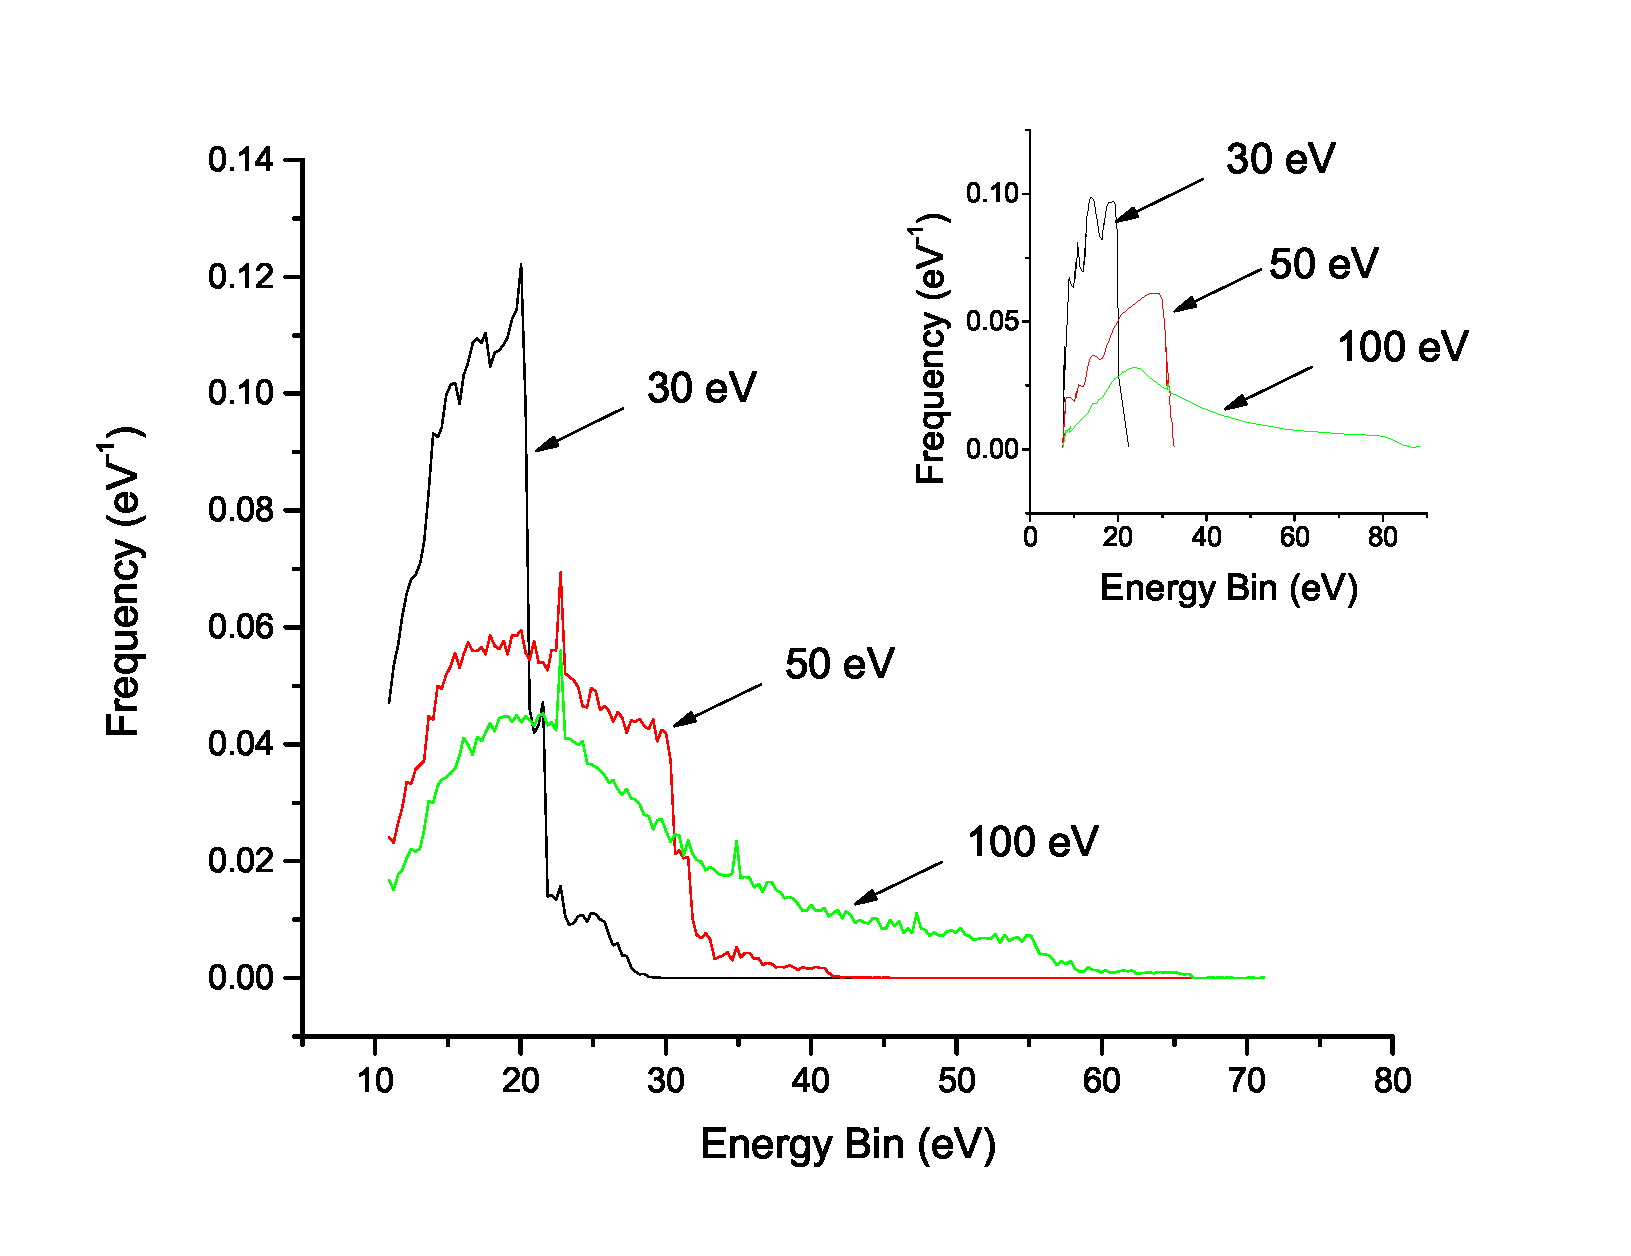
\includegraphics[width=\textwidth]{SingleCollsionEnergyLoss_Turner}
    \caption{Single Collision Energy Loss in Water\cite{turner_comparative_1982}}
  \end{figure}
\vspace{2mm}
Discrepancies are in the resolution of cross section data
\end{frame}
%%%%%%%%%%%%%%%%%%%%%%%%%%%%%%%%%%%%%%%%%%%%%%%%%%%%%%%%%%%%%%%%%%%%%%%%%%
\begin{frame}{Example Event}
  \begin{figure}
    \includegraphics[height=0.75\textheight]{GEANT4AnnotatedGeo_EnergyDepEvent}
  \end{figure}
\end{frame}
%%%%%%%%%%%%%%%%%%%%%%%%%%%%%%%%%%%%%%%%%%%%%%%%%%%%%%%%%%%%%%%%%%%%%%%%%%

\input{doc/LightYeildEDep}
\input{doc/ScintillationSlab}
\input{doc/RangeSim}
\input{doc/EnergyDepTracking}
\input{doc/LightQuenching}
\input{doc/ElectronEnergyDeposition}
\input{doc/GS20Calibration}
\input{doc/DetectorSim}
\input{doc/ParticleTracks}
\input{doc/PSCalibration}
\input{doc/MCNPXRPMModels}


    %%%%%%%%%%%%%%%%%%%%%%%%%%%%%%%%%%%%%%%%%%%%%%%%%%%%%%%%%%%%%%%%%%%%%%%%%%%
    % A VITA IS REQUIRED
    %%%%%%%%%%%%%%%%%%%%%%%%%%%%%%%%%%%%%%%%%%%%%%%%%%%%%%%%%%%%%%%%%%%%%%%%%%%
    \addToTOC{Vita}
    \chapter*{Vita} \label{ch:vita}
Matthew J. Urffer was born January, 29, 1988 on a small turkey farm on Urffer Road in Coopersburg, Pa.
He got his B.S. in physics from Carnegie Mellon University in Pittsburgh, PA. 
Upon graduation Matthew enrolled at the University of Tennessee, Knoxville where he received his Masters in Nuclear Engineering in December, 2012 and is currently pursuing a doctorate in nuclear engineering.

\end{document}
